\chapter{Theory}\label{chap:theory}

The Standard Model (SM) of particle physics describes interactions between all known elementary particles via the strong, weak, and electromagnetic forces. It is capable of making astonishingly precise and accurate predictions. For example, the prediction and measurement of the anomalous magnetic dipole moment of the electron agree to one part in $10^{12}$~\cite{Fan:2022eto}. Furthermore, measurements made of high energy collisions, like those at the LHC, remain consistent with SM predictions. However, the SM cannot explain several key observations, including dark matter~\cite{Clowe:2006eq}, neutrino oscillations~\cite{Super-Kamiokande:1998kpq}, and the matter-antimatter asymmetry of the universe~\cite{Canetti:2012zc}. It is anomalies like these that motivate the formulation of theories that go beyond the SM.

Anomalous observations are not the only source of motivation when developing new theories. There are also theoretical problems with the SM such as the hierarchy problem~\cite{Thomson:2013zua} and that the SM does not include a description of gravity. From a scientific perspective, a BSM theory does not need to solve these problems, it only needs to provide predictions that accurately describe our measurements. However, history teaches us that when pursuing solutions to theoretical problems, we can also make scientific breakthroughs. The prediction of the charm quark in 1970~\cite{Glashow:1970gm} before its discovery in 1975~\cite{Cazzoli:1975et} is a great example of this.

This chapter begins with an explanation of the SM, starting with the particle content and the allowed interactions before moving onto a mathematical description of the theory. Following this, the content is tailored towards the results discussed later in this thesis, those being the di-Higgs search in \cref{chap:dihiggs} and the Effective Field Theory (EFT) interpretation in \cref{chap:eft}. This content includes Higgs boson phenomenology at the LHC and relevant extensions to the SM, including EFTs and two BSM theories that motivate the search in \cref{chap:dihiggs}, namely Warped Extra Dimensions (WED) and the Next-to-Minimal Supersymmetric Standard Model (NMSSM).

\section{The Standard Model of Particle Physics}\label{sec:sm}

The SM is formulated as a relativistic quantum field theory (QFT) where each particle in the theory is represented by its own field and excitations of those fields are then the physical particles that we observe in nature. Particles can interact with each other via the exchange of a subset of SM particles called \textit{force carriers}. The types of allowed interactions and their corresponding strengths are encoded in a Lagrangian density, \LSM, together with the particle properties (mass and spin). 

\subsection{Particle Content}
A schematic of the SM particle content, including every SM particle with its properties and categorizations is provided in \cref{fig:sm_particle_content}. The particle content can be initially categorized into two groups: spin-$\frac{1}{2}$ fermions which are matter constituents, and spin-integer bosons which are force carriers and are spin-1 except for the Higgs boson which is spin-0. 

There are four spin-1 bosons in the SM: the photon ($\gamma$) which mediates the electromagnetic force, the \PWpm and \PZ bosons which mediate the weak force, and the gluon (\Pg) which mediates the strong force. Particles that interact with photons carry \textit{electric charge}; particles that interact with gluons carry a \textit{colour charge}, which comes in three possible states: $r$, $g$ and $b$, and particles that interact with \PWpm and \PZ bosons carry charges called \textit{weak isospin} and/or \textit{weak hypercharge}. More details on these charges are given in \cref{sec:sm_lagrangian}.

The fermions are split by those that interact with the strong force, called \textit{quarks}, and those that do not, called \textit{leptons}. Leptons are further split into those which are electrically charged ($l$), and those which are not, called \textit{neutrinos} ($\nu$).  Quarks are similarly split by electric charge into up-type quarks and down-type quarks, with charge $\frac{2}{3}$ and $-\frac{1}{3}$ respectively (in units of elementary charge, $e$). 

The fermions can be also categorized into three generations based on a mass hierarchy, where the first generation is the least massive. Each generation contains an up-type quark, a down-type quark, a charged lepton, and a neutrino. The first generation contains the main constituents of the visible matter in the universe, those being the up and down quarks, and the electron. Additionally, all charged fermions have a corresponding antiparticle which has the same mass but opposite charge and parity.

The remaining particle is the Higgs boson which plays a special role in the SM. We will see later on that its introduction to the model is necessary to correctly describe the distribution of masses for particles in the theory. 

\begin{figure}
  \centering
  \hbox{\hspace{-2.5cm}\resizebox{1.2\textwidth}{!}{\inputtikz{Figures/Theory/SM/particle_content.tex}}}
  \caption[SM Particle Content]{Particle content of the SM. The mass, electric charge, colour and spin are given for each particle. All masses are taken from Ref.~\cite{ParticleDataGroup:2020ssz} except the Higgs boson mass which is taken from Ref.~\cite{CMS:2020xrn}.}\label{fig:sm_particle_content}
\end{figure}
\subsection{Interactions}
The electromagnetic and weak forces are described together by a single force: the \textit{electroweak} force. Particles that interact via the electroweak force include all fermions and the electroweak bosons: \PZ, \PW, $\gamma$ and \PH (all bosons except the gluon). Feynman diagram vertices for these interactions are given in \cref{fig:electroweak_fermion_vertices}. All fermions can interact via the exchange of \PZ boson and all left-handed particles/right-handed anti-particles can interact via the exchange of a \PW boson. All electrically charged fermions can interact via the exchange of a photon and all massive fermions can interact with the Higgs boson. The three and four-point interactions involving only electroweak bosons, shown in \cref{fig:electroweak_3_point_boson_vertices,fig:electroweak_4_point_boson_vertices}, are also allowed. In the strong force, quarks and gluons interact with each other according to the Feynman diagram vertices shown in \cref{fig:strong_vertices}.

\begin{figure}[b!]
  \centering
  \inputtikz{Figures/Theory/SM/ffz.tex}
  \inputtikz{Figures/Theory/SM/ffa.tex}
  \inputtikz{Figures/Theory/SM/ffh.tex} \\
  \inputtikz{Figures/Theory/SM/fnuw.tex}
  \inputtikz{Figures/Theory/SM/udw.tex}
  \caption[Electroweak Feynman Diagram Vertices]{Feynman diagram vertices allowed in the SM involving electroweak interactions with fermions. Interactions with a photon, \PZ boson, or a Higgs boson, require the fermion ($f$) flavour to be the same. Massive fermions are denoted by $f_m$ and exclude neutrinos. Interactions with \PW bosons can involve fermions from different generations and must involve either a lepton ($l$) and a neutrino ($\nu$) or an up-type quark ($u$) and a down-type quark ($d$). The $L$ and $R$ subscripts denote left-handed and right-handed fermions respectively. Charged-conjugated versions of the \PW-interaction diagrams are also possible if the handedness is reversed.}\label{fig:electroweak_fermion_vertices}
\end{figure} 


\begin{figure}
  \centering
  \inputtikz{Figures/Theory/SM/wwz.tex}
  \inputtikz{Figures/Theory/SM/wwh.tex}
  \inputtikz{Figures/Theory/SM/zzh.tex}
  \inputtikz{Figures/Theory/SM/hhh.tex}
  \caption[Three-Point Electroweak Boson Feynman Diagram Vertices]{Feynman diagram vertices allowed in the SM involving three electroweak bosons.}\label{fig:electroweak_3_point_boson_vertices}
\end{figure}

\begin{figure}
  \centering
  \inputtikz{Figures/Theory/SM/wwzz.tex}
  \inputtikz{Figures/Theory/SM/wwww.tex} \\
  \inputtikz{Figures/Theory/SM/wwhh.tex}
  \inputtikz{Figures/Theory/SM/hhhh.tex}
  \caption[Four-Point Electroweak Boson Feynman Diagram Vertices]{Feynman diagram vertices allowed in the SM involving four electroweak bosons.}\label{fig:electroweak_4_point_boson_vertices}
\end{figure}

\begin{figure}
  \centering
  \inputtikz{Figures/Theory/SM/qqg.tex}
  \inputtikz{Figures/Theory/SM/ggg.tex}
  \inputtikz{Figures/Theory/SM/gggg.tex}
  \caption[Strong Feynman Diagram Vertices]{Feynman diagram vertices allowed in the SM that involve a strong interaction. On the left, $q$ refers to a quark (or antiquark) of the same flavour.}\label{fig:strong_vertices}
\end{figure}
\subsection{Quantum Field Theory}\label{sec:electroweak}
The SM can be described by a Lagrangian density, \LSM, which is a function of the particle fields and their derivatives. By applying the Euler-Lagrange equations to \LSM, we can then derive equations of motion that describe the dynamics and interactions of these fields. In this section, concepts related to QFT that will help to understand the construction of \LSM will be described. In the rest of this section, Lagrangian densities will be represented by $\mathcal{L}$ and referred to as ``Lagrangians'' (omitting ``density'').

\subsubsection{Real Scalar Fields}
One of the simplest particle theories one could write down consists of a single Lorentz real scalar field, $\phi(x,y,z,t)$, with a Lagrangian:
\begin{equation}
  \mathcal{L} = \frac{1}{2}\partial_\mu \phi \partial^\mu \phi - \frac{1}{2}m^2\phi^2
\end{equation}
and after applying the Euler-Lagrange equations:
\begin{equation}
  0 = \frac{\partial \mathcal{L}}{\partial \phi} - \partial_\mu \frac{\partial \mathcal{L}}{\partial(\partial_\mu \phi)}
\end{equation}
this becomes:
\begin{equation}
  0 = \partial_\mu \partial^\mu \phi + m^2 \phi \label{eq:klein_gordon}
\end{equation}
which can be identified as a relativistic wave equation, namely the Klein-Gordon equation, which describes a particle with mass $m$. In this theory, the particles are non-interacting. To introduce interactions, we need to add terms that are higher orders of \phi, for example:
\begin{equation}
  \mathcal{L} = \frac{1}{2}\partial_\mu \phi \partial^\mu \phi - \frac{1}{2}m^2\phi^2 + \lambda_3 \phi^3 + \lambda_4 \phi^4
  \label{eq:scalar4}
\end{equation}
where $\lambda_3 \phi^3$ and $\lambda_4 \phi^4$ correspond to three-point and four-point interactions respectively. Generally, a term containing greater than two fields, including powers of the same field, corresponds to an interaction involving that combination of fields. Adding terms that have powers of $\phi$ greater than four are not allowed if one wants a renormalizable theory, i.e.\ a theory that has finite predictions at arbitrarily high energy scales~\cite{Peskin:1995ev}. Strictly speaking, a renormalizable Lagrangian must have dimensions $[\mathcal{L}] = \mathrm{GeV}^4$. Given that $[\partial_\mu \phi] = \mathrm{GeV}^2$, $[\phi] = \mathrm{GeV}$ and $[m] = \mathrm{GeV}$, this is satisfied in \cref{eq:scalar4}. 

\newpage

\noindent
Regardless of renormalizability, a Lagrangian must additionally:
\begin{enumerate}
  \item be real since the action, $S$, which is an integral over the Lagrangian, must be real;
  \item be a local function of the fields and their derivatives calculated at the same spacetime point;
  \item be invariant under any symmetries of the theory.
\end{enumerate}
\Cref{eq:scalar4} is invariant under Poincar\'e transformations, which include translations and rotations in space, as well as Lorentz boosts. According to Noether's theorem, a continuous symmetry has a corresponding conservation law and in the case of Poincar\'e transformations, the conserved quantities are energy, momentum, and angular momentum. The full SM Lagrangian has additional symmetries which will be highlighted throughout the rest of this section.

Lorentz invariance is an assumed requirement for all Lagrangians in this chapter. The condition on renormalization is also required except for effective field theories which will be discussed in \cref{sec:EFT}. 

\subsubsection{Vector Fields}
In the SM, the spin-1 force carriers are represented by vector fields. The most general Lagrangian that is Lorentz invariant and contains a real vector field is:
\begin{equation}
  \mathcal{L} = aS^2 + b F_\mn F^\mn + c G_\mn G^\mn + d A_\mu A^\mu
\end{equation}
where:
\begin{align}
  S &= \partial_\mu A^\mu,\quad &&\text{is a Lorentz scalar}; \\
  F_\mn &= \partial_\mu A_\nu - \partial_\nu A_\mu,\quad &&\text{is an antisymmetric rank 2 tensor}; \label{eq:fmn} \\
  G_\mn &= \partial_\mu A_\nu + \partial_\nu A_\mu - \frac{1}{2} \eta_\mn S,\quad &&\text{is a symmetric and traceless rank 2 tensor};
\end{align}
and $a, b, c$ and $d$ are arbitrary constants. If we want the Lagrangian to also be gauge invariant, meaning that it is invariant under transformations of the form:
\begin{equation}
  A_\mu \to A_\mu - \partial_\mu \lambda
  \label{eq:gauge_transformation}
\end{equation}
where $\lambda$ is an arbitrary scalar function of spacetime, only one of the terms is viable and the most general Lagrangian is:
\begin{equation}
  \mathcal{L} = F_\mn F^\mn .
\end{equation}
This is the Maxwell Lagrangian for the free electromagnetic field.

\subsubsection{Complex Scalar Fields}
Returning to scalar fields but now considering the field to be complex, the most general Lagrangian becomes:
\begin{equation}
  \mathcal{L} = \partial_\mu \phi^* \partial^\mu \phi - V(\phi^*\phi)
  \label{eq:scalar_complex}
\end{equation}
where the potential, $V(\phi^*\phi)$, is a polynomial of order two or less. The three-point interaction term is now missing due to the requirement that $\mathcal{L}$ be real, and the Lagrangian has a new symmetry compared to the real scalar field Lagrangian. The Lagrangian is now invariant under the rotation of a complex phase:
\begin{equation}
  \phi(x) \to e^{i\theta}\phi(x)
\end{equation}
where $\theta$ is a real number. The symmetry is called \textit{Abelian} because the transformations commute:
\begin{equation}
  e^{-i\theta_1}e^{-i\theta_2} = e^{-i\theta_2}e^{-i\theta_1},
\end{equation}
and is called a \textit{global symmetry} because the same transformation is applied at all points in spacetime, i.e.\ $\theta$ is a constant. 

The Lagrangian of \Cref{eq:scalar_complex} is not invariant under a local transformation of the type:
\begin{equation}
  \phi(x) \to e^{i\theta(x)} \phi(x)
  \label{eq:local_transformation}
\end{equation}
but an invariant Lagrangian can be created if a new vector field, $A_\mu$, is introduced which simultaneously transforms as 
\begin{equation}
  A_\mu(x) \to A_\mu(x) - \frac{1}{e}\partial_\mu \theta(x)
  \label{eq:gauge_transformation_2}
\end{equation}
which is the same as the gauge transformation in \cref{eq:gauge_transformation} where $\lambda = \theta(x)/e$. The simultaneous transformation of $\phi$ and $A_\mu$ is referred to as a \textit{local gauge} transformation and the new vector field is known as a \textit{gauge field}. The Lagrangian is given by:
\begin{equation}
  \mathcal{L} = (D_\mu\phi)^* D^\mu \phi - V(\phi^*\phi)
  \label{eq:scalar_complex_gauge}
\end{equation}
where the covariant derivative, $D_\mu$, is defined as:
\begin{equation}
  D_\mu \phi \equiv \partial_\mu \phi + ieA_\mu \phi.
\end{equation}
Now adding the $F_\mn F^\mn$ term (\cref{eq:fmn}), we arrive at the most general gauge invariant Lagrangian for a complex scalar field:
\begin{equation}
  \mathcal{L} = F_\mn F^\mn + (D_\mu\phi)^* D^\mu \phi - V(\phi^*\phi) .
\end{equation}

In the SM, local gauge symmetries are imposed on the Lagrangian which give rise to the existence of vector bosons, which are the force carriers: the gluons, photon, and the \PWpm and \PZ bosons. Given that they are related to gauge transformations, the force carriers are also referred to as \textit{gauge bosons}.

\subsubsection{Non-Abelian Gauge Fields}
The simultaneous transformation of $\phi$ and $A_\mu$ in \cref{eq:local_transformation,eq:gauge_transformation_2} is a \U{1} transformation. When generalizing to \U{N}, the Lagrangian in \cref{eq:scalar_complex_gauge} becomes:
\begin{equation}
  \mathcal{L} = (D_\mu\phi)^\dag D^\mu \phi - V(\phi^\dag\phi)
\end{equation}
where $\phi$ and $A_\mu$ transform as
\begin{align}
  \phi &\to M \phi \\
  A_\mu &\to M A_\mu M^\dag + \frac{i}{g}(\partial_\mu M)M^\dag \label{eq:non_abelian_vector_transformation}
\end{align}
where $M(x)$ is an element of the \U{N} group. \Cref{eq:non_abelian_vector_transformation} holds if $A_\mu$ is an element of the Lie algebra, meaning that it can be written as $A_\mu = A_\mu^a T^a$ where $A_\mu^a$ are real constants, $T^a$ are the generators of some representation of the Lie algebra, and $a \in \{1,\ldots,D\}$ where $D=N^2$ is the dimensionality of \U{N}. Therefore, imposing a local \U{N} symmetry has lead to the introduction of $D$ gauge bosons, where each gauge boson is represented by a component, $A_\mu^a$. 

In the non-Abelian case, the $F_\mn F^\mn$ term is no longer gauge invariant. In an attempt to find a similar term that \textit{is} gauge invariant, we redefine $F_\mn$ as:
\begin{align}
  F_\mn &= -\frac{i}{g} [D_\mu, D_\nu] \\
  &= \partial_\mu A_\nu - \partial_\nu A_\mu + ig[A_\mu, A_\nu]
\end{align}
which is still consistent with the Abelian case since $[A_\nu, A_\nu]$ would be zero. With this definition, $F_\mn F^\mn$ is still not invariant, but its trace is. Therefore, the most general scalar field Lagrangian with a \U{N} gauge symmetry is:
\begin{equation}
  \mathcal{L} = -\frac{1}{2} \Tr F_\mn F^\mn + (D_\mu\phi)^\dag D^\mu \phi - V(\phi^\dag\phi).
\end{equation}

Writing the first term alone and in terms of the gauge field components, $A_\mu^a$, we find:
\begin{align}
  \mathcal{L} = &-\frac{1}{2} \Tr F_\mn F^\mn = - \frac{1}{4} F_\mn^a F^{\mn a} \\
  &= -\frac{1}{4} (\partial_\mu A_\nu^a - \partial_\nu A_\mu^a) (\partial_\nu A^a_\mu) (\partial^\mu A^{\nu a} - \partial^\nu A_{\mu a}) (\partial_\nu A^a_\mu) \\
  &+ \frac{g}{2} f^{abc} (\partial_\mu A^a_\nu - \partial_\nu A^a_\mu) A^{\mu b}A^{\nu c} - \frac{g^2}{4} f^{abc} f^{ade} A_\mu^b A_\nu^c A^{\mu d} A^{\nu e}
\end{align}
where the last two terms represent three-point and four-point interactions of the gauge bosons, in an analogous way to \cref{eq:scalar4}. 

The conclusions reached here about non-abelian gauge fields apply to any subset of \U{N}, including \SU{N} groups which are seen in the SM.

\subsubsection{Spinors}
In addition to the Klein-Gordon equation (\cref{eq:klein_gordon}), particles that have spin $\frac{1}{2}$ must also satisfy the Dirac equation:
\begin{equation}
  i \gamma^\mu \partial_\mu \psi - m \psi = 0
\end{equation}
where $m$ is the mass of the particle, $\psi$ is the particle field, and $\gamma^\mu$ are the $4\times4$ gamma matrices~\cite{Thomson:2013zua}. 

A Lorentz scalar that can be constructed out of spinor fields is $\bar{\psi} \psi$ where we have introduced the Dirac adjoint, $\bar{\psi}$, as: 
\begin{equation}
  \bar{\psi} \equiv \psi^\dag \gamma^0 .
\end{equation}
For any pair of spinors, $\psi$ and $\chi$, $\bar{\psi} \gamma^\mu \chi$ is a Lorentz vector, and for any Lorentz vector, $a_\mu$, $\bar{\psi} \slashed{a} \chi$ is a Lorentz scalar where we have introduced the Dirac slash notation:
\begin{equation}
  \slashed{a} \equiv \gamma^\mu a_\mu .
\end{equation}
This also applies when the vector is a derivative so $\bar{\psi}\slashed{\partial}\psi$ is also a Lorentz scalar.

In the SM, spinors are decomposed into their left and right-handed components. To define these components, we first introduce a fifth gamma matrix:
\begin{equation}
  \gamma^5 = i\gamma^0 \gamma^1 \gamma^2 \gamma^3 .
\end{equation}
The left/right-handed component of a spinor, $\psi_{L/R}$, is given by $P_{L/R} \psi$ where:
\begin{equation}
  P_L = \frac{1}{2} (\iden - \gamma^5) \text{ and } P_R = \frac{1}{2}(\iden + \gamma^5) .
\end{equation}
Under a parity transformation, a left/right-handed spinor transforms as:
\begin{equation}
  \psi_{L/R} \to \gamma^0 \psi_{L/R}
\end{equation}
and it can be shown that $P_{L/R} (\gamma^0 \psi_{L/R}) = 0$, i.e.\ a parity transformation changes a left-handed spinor into a right-handed spinor and a right-handed spinor into a left-handed spinor. Given this transformation property, we can create a parity-violating theory by writing a Lagrangian that has different terms for $\psi_L$ than for $\psi_R$. This will be essential in describing the weak interaction that behaves differently with left and right-handed fermions.

\subsubsection{Spontaneous Symmetry Breaking}
So far, we have interpreted a field, $\phi$, in a Lagrangian as the field of a physical particle. This has the implicit assumption that a field value of zero corresponds to the vacuum state of the Lagrangian, i.e.\ the state with the lowest energy. However, this need not be the case. Consider the complex scalar Lagrangian of \cref{eq:scalar_complex}, which has a global \U{1} symmetry, with the potential:
\begin{equation}
  V(\phi^*, \phi) = m^2 \phi^*\phi + \frac{1}{2}\lambda (\phi^*\phi)^2 .
  \label{eq:scalar_complex_potential}
\end{equation}
\begin{figure}
  \centering
  \scalebox{1.5}{
   \inputtikz{Figures/Theory/SM/sombrero.tex}
  }
  \caption[Higgs Field Potential]{The potential of a complex scalar field, $V(\phi) = m^2 \phi^*\phi + \frac{1}{2}\lambda (\phi^*\phi)^2$, where $m^2 < 0$ and $\lambda > 0$.}\label{fig:sombrero}
\end{figure}
If $m^2 < 0$ and $\lambda > 0$, then the potential will look like that shown in \cref{fig:sombrero} and have a circle of minima in the complex plane at:
\begin{equation}
  \phi = \frac{v}{\sqrt{2}}e^{i\theta},\quad \theta \in [0, 2\pi]
  \label{eq:phi_vacuum_state}
\end{equation}
where we have used the conventions, $\mu^2 = -m^2$ and $v = \mu / \sqrt{\lambda}$, where $v$ is real and referred to as the \textit{vacuum expectation value} (vev). We can choose a particular minimum, $\phi = \phi_0 = v / \sqrt{2}$, and expanding around this vacuum state we get:
\begin{alignat}{2}
  \phi (x) &= \frac{1}{\sqrt{2}} (v + \rho(x) ), \quad &&\rho \in \mathbb{C} \\
  &= \frac{1}{\sqrt{2}} (v + \varphi (x) + i \chi (x) ), \quad &&\varphi,\chi \in \mathbb{R}
\end{alignat}
and the potential becomes:
\begin{equation}
  V(\phi^*, \phi) = -\frac{\mu^4}{2\lambda} + \mu^2 \varphi^2 + \frac{1}{2} \lambda v \varphi (\varphi^2 + \chi^2) + \frac{1}{8} \lambda (\varphi^2 + \chi^2)^2
  \label{eq:scalar_complex_potential_expanded}
\end{equation}
where the second term is a mass term for $\varphi$ and there are no mass terms for $\chi$. By expanding around the vacuum state, we have revealed the physical particle spectrum for this Lagrangian, which is two scalar particles, $\varphi$ and $\chi$, where $m_\varphi = \sqrt{2}\mu$ and $\chi$ is massless. The massless scalar particle is known as a Goldstone boson.



This Lagrangian is invariant under a global \U{1} transformation: $\phi \to e^{i\theta} \phi$, but since $e^{i\theta}\phi_0 \neq \phi_0$, this does not correspond to the analogous transformation: $\rho \to e^{i\theta} \rho$. We therefore say that the global \U{1} symmetry is \textit{spontaneously broken}. The original symmetry is still present, but not apparent now that the Lagrangian is written in terms of the physical particle fields. 

We can now generalize to theories that are invariant under any symmetry group, $G$, whereby the field transforms as $\phi \to M \phi$, where $M$ is an element of the group. The symmetry is spontaneously broken if $M \phi_0 \neq \phi_0$ for any $M$, or unbroken if $M \phi_0 = \phi_0$ for all $M$. Considering an infinitesimal transformation of $\phi_0$:
\begin{equation}
  \phi_0 \to \phi_0 + i \theta^a T^a \phi_0
\end{equation}
where $T^a$ are the generators of the group, and $\theta^a$ are infinitesimally-small real constants, we identify broken generators as ones where $T \phi_0 \neq \phi_0$ and unbroken generators as ones where $T \phi_0 = \phi_0$. The set of unbroken generators corresponds to a \textit{residual symmetry group}, $H$, which is a subgroup of the original group. 

When $T \phi \neq 0$ for all $T$, there may still exist linear combinations of the generators, $\hat{T}=c^a T^a$ where $\hat{T} \phi_0 = 0$. To determine these linear combinations, we first define the symmetry breaking matrix:
\begin{equation}
  S^{ab} = \phi_0^\dag \{T^a, T^b\} \phi_0 .
  \label{eq:symmetry_breaking_matrix}
\end{equation}
For \U{N} and \SU{N} symmetry groups where $T^a$ are Hermitian, $S^{ab}$ is real and symmetric and therefore has $D$ real eigenvectors, $c_i$, with eigenvalues $\lambda_i$. It can be shown that a new generator defined as $\hat{T}^i = c_i^a T^a$, is an unbroken generator when $\lambda_i = 0$, and a broken generator when $\lambda_i \neq 0$. It can be further shown that every broken generator gives rise to a massless Goldstone particle. This is known as Goldstone's theorem~\cite{Goldstone:1962es} and holds for theories with global symmetries. To determine the particle spectra of a gauge theory, we turn to the Higgs mechanism.

\subsubsection{The Higgs Mechanism}
Consider the Lagrangian of \cref{eq:scalar_complex_gauge}, which has a local \U{1} symmetry, with the same potential as \cref{eq:scalar_complex_potential}. Now that the vector field, $A^\mu$, is introduced, the vacuum state is specified by values of $A^\mu$ and $\phi$ simultaneously. In the temporal gauge ($A^0 = 0$), this is given by \cref{eq:phi_vacuum_state} and $A_\mu = 0$.
  
Once again expanding the scalar field as $\phi = (v + \varphi + i \chi) / \sqrt{2}$, we regain the same potential as \cref{eq:scalar_complex_potential_expanded} and new terms from the expansion of $F_\mn F^\mn$ and $(D_\mu \phi)^* D^\mu \phi$. Writing only the quadratic terms and transforming to the unitary gauge ($\theta(x) = -\chi / v$) we find:
\begin{equation}
  \mathcal{L} = F_\mn F^\mn + \frac{1}{2} e^2 v^2 A_\mu A^\mu + \frac{1}{2} \partial_\mu \varphi \partial^\mu \varphi - \mu^2 \varphi^2 + \cdots
\end{equation}
where we can identify two distinct fields, $A_\mu$ and $\phi$, which have masses $\sqrt{2}\mu$ and $ev$ respectively. As in the global case, the \U{1} symmetry is broken, but unlike the global case, the symmetry breaking has not led to any massless particles. Instead, the originally-massless vector boson has been given a mass.

When generalizing to theories that are invariant under any symmetry group, a similar conclusion is found. If there are $D$ generators of the group, where $D^'$ are broken, then there are $D^'$ massive vector particles and $D-D^'$ massless vector bosons. In the SM, this is the mechanism by which the gauge bosons of the weak force, \PWpm and \PZ, acquire mass. 
\subsection{The Standard Model Lagrangian}\label{sec:sm_lagrangian}
\subsubsection{Quantum Electrodynamics}
The QFT of electromagnetism is known as quantum electrodynamics (QED). It describes the interaction between charged fermions and photons which are represented by a spinor, $\psi$, and a vector field, $A^\mu$, respectively. The QED Lagrangian is:
\begin{equation}
  \LQED = -\frac{1}{4} F_\mn F^\mn +  \bar{\psi} (i \slashed{D} - m)\psi,
\end{equation}
and is invariant under global and local \U{1} transformations which lead to the conservation of particle number and electric charge respectively. It also is symmetrical under parity, charge conjugation, and time reversal transformations. However, experiments have shown that parity symmetry is only approximate, and can be violated~\cite{Wu:1957my}. Therefore, the QED Lagrangian does not sufficiently describe the behaviour of charged fermions in nature. In the SM, parity violation is introduced via the weak force which couples only to left-handed fermions.

We can start to consider how we can introduce parity violation by writing the fermionic components of the QED Lagrangian in terms of the left and right-handed components of the fermion:
\begin{equation}
  \LQED = \bar{\psi}_L i \slashed{\partial} \psi_L + \bar{\psi}_R i \slashed{\partial} \psi_R - m (\bar{\psi}_L \psi_R + \bar{\psi}_R \psi_L) .
\end{equation}
If the fermion is massless, then the left-handed and right-handed components are decoupled from each other and we can write a Lagrangian containing only a left-handed spinor:
\begin{equation}
  \mathcal{L} = \bar{\psi}_L i \slashed{\partial} \psi_L + \cdots
\end{equation}
which would be parity-violating. Therefore, parity violation can be introduced by treating left-handed and right-handed fermions differently in the SM, and this is done in electroweak theory which supersedes QED as a description of electromagnetism and describes the weak interaction at the same time.

\subsubsection{Quantum Chromodynamics}
The QFT of the strong interaction is known as quantum chromodynamics (QCD). The Lagrangian is required to be invariant under local \SU{3} transformations which implies the existence of eight gauge bosons called gluons. The Lagrangian is given by:
\begin{equation}
  \LQCD = \sum_f i \bar{\psi}^f_i (\slashed{D}_{ij} -m^f \delta_{ij})\psi^f_j - \frac{1}{4} G^{c\mn} G^c_\mn
  \label{eq:qcd_lagrangian}
\end{equation}
and the covariant derivative is written as:
\begin{equation}
  (D_\mu)_{ij} = \partial_\mu \delta_{ij} + i g_s G^c_\mu \frac{\lambda^c_{ij}}{2}
\end{equation}
where the strength of the interaction is characterized by $g_s$, the gluons are represented by $G^a_\mu$, and $\lambda^c$ are the Gell-Mann matrices which are a set of $3\times3$ matrices that generate \SU{3}~\cite{Thomson:2013zua}. The quark spinors are given by $\psi^f_i$ where $f \in \{u, d, c, s, t, b\}$ corresponds to a quark \textit{flavour} and $i \in \{r, g, b\}$ corresponds to a quark \textit{colour}. 

Since the \SU{3} symmetry is non-abelian, the gluons are self-interacting and this has profound consequences for the strong interaction. Firstly, $g_s$ increases as the energy scale of an interaction decreases (see \cref{fig:alphas_running}) which is opposite to the behaviour seen in the electromagnetic interaction where there are no self-interactions. This means that at energy scales below $O(1\GeV)$ where $g_s \sim 1$, calculations using perturbation theory are no longer possible, making predictions from QCD more challenging. Fortunately, for energies $O(>100\GeV)$ such as those probed by the LHC, $g_s \sim 0.1$ and perturbation theory is applicable.

A further consequence of gluon self-interactions is the concept of colour confinement which means that quarks and gluons cannot be observed as isolated free particles. Instead, they must exist within colourless bound states called hadrons. States with even and odd numbers of quarks are called mesons and baryons respectively. The two-quark and three-quark variants of these states are commonly produced by QCD interactions at the LHC, and states with higher than three quarks such as tetraquarks and pentaquarks have also been observed~\cite{Liu:2019zoy}.

\begin{figure}
  \centering
  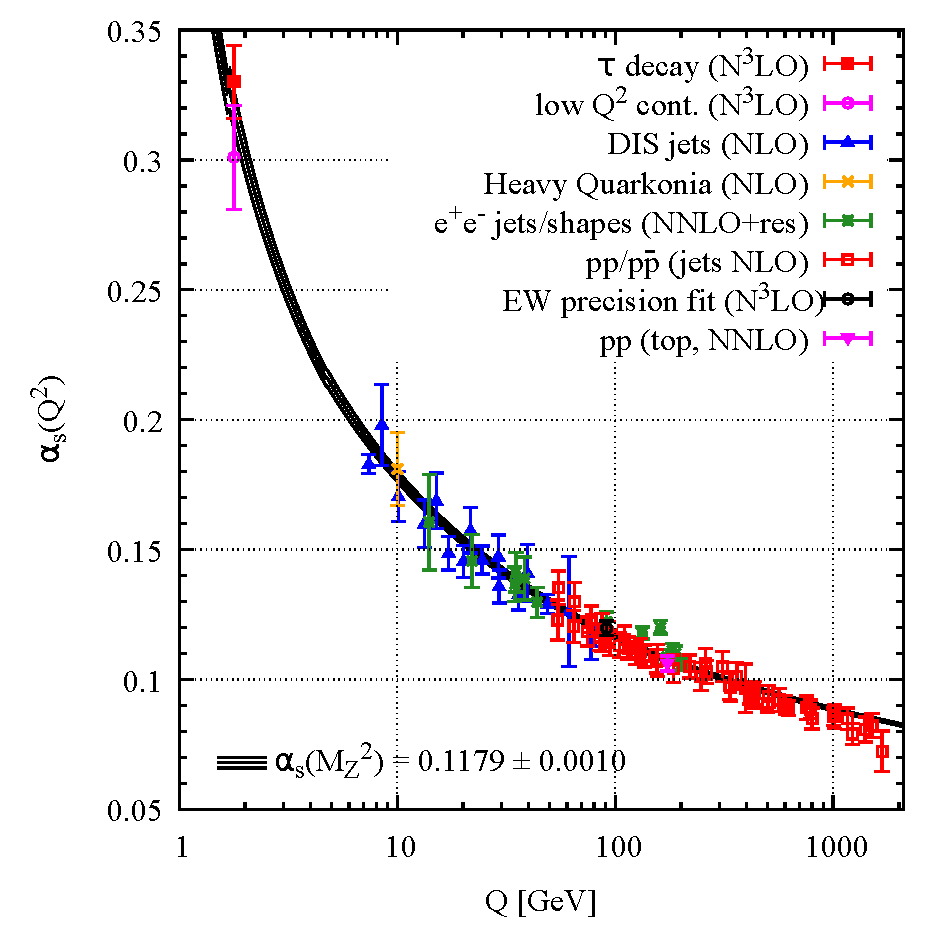
\includegraphics[width=0.7\textwidth]{Figures/Theory/SM/alphas_running.pdf}
  \caption[Measurements of $\alpha_s$ as a Function of Energy Scale]{Summary of measurements of $\alpha_s$ ($\alpha_s = g_s^2 / 4\pi$) as a function of the energy scale, $Q$, taken from Ref.~\cite{ParticleDataGroup:2020ssz}. Each set of coloured points corresponds to a different set of measurements and the degree of QCD perturbation theory used to extract $\alpha_s$ is indicated by the brackets in the legend. Further details about the measurements and $\alpha_s$ calculations can be found in Ref.~\cite{ParticleDataGroup:2020ssz}.}\label{fig:alphas_running}
\end{figure}

\subsubsection{Electroweak Gauge Theory}
In the SM, the electroweak bosons arise from an $\SU{2} \times \U{1}$ gauge symmetry of \LSM. The representation of some field, $\chi$, under \SU{2} is given by generators $\{T^a\}$, $a \in \{1,2,3\}$, and the generator of \U{1} can be any real number, $Y$, such that a gauge transformation is given by:
\begin{equation}
  \chi \to e^{i\theta^a T^a + i\eta Y} \chi
\end{equation}
where $\theta^a$ and $\eta$ are real numbers. The generators $T^a$ and $Y$ are called \textit{weak isospin} and \textit{weak hypercharge} respectively. The covariant derivative is given by:
\begin{equation}
  D_\mu = \partial_\mu + i g_2 A^a_\mu T^a + i g_1 Y B_\mu
  \label{eq:electroweak_covariant}
\end{equation}
where $A^a_\mu$ and $B_\mu$ are the \SU{2} and \U{1} gauge fields respectively. 

Experiments have measured the mass of the \PW and \PZ bosons to be non-zero~\cite{ParticleDataGroup:2020ssz} and in the SM, these masses are introduced via the Higgs mechanism. This necessitates electroweak theory to include a complex scalar field, $\phi$, which is the \textit{Higgs field}, and is in the fundamental representation of \SU{2} and $Y = 1/2$. By defining a fourth generator:
\begin{equation}
  t^4 = \frac{g_1}{2g_2} \iden,
\end{equation}
and $A_\mu^4 = B_\mu$, the gauge fields can be represented by a single vector field in the covariant derivative of the Higgs field:
\begin{equation}
  D_\mu \phi = \partial_\mu \phi + i g_2 A_\mu^{a'} t^{a'} \phi,
\end{equation}
which is useful for applying the ideas of the symmetry breaking matrix introduced in \cref{eq:symmetry_breaking_matrix}. The Lagrangian of the theory is:
\begin{equation}
  \mathcal{L} = -\frac{1}{2} \Tr W_\mn W^\mn - \frac{1}{4} F_\mn F^\mn + (D_\mu \phi)^\dag D^\mu \phi + \mu^2 \phi^\dag \phi - \lambda (\phi^\dag \phi)^2 
  \label{eq:electroweak_gauge_terms}
\end{equation}
where $W_\mn$ and $F_\mn$ are the field strength tensors of the \SU{2} and \U{1} gauge fields respectively. After electroweak symmetry breaking, the residual symmetry group is \U{1} and in terms of the original gauge fields, the physical gauge boson spectrum is:
\begin{align}
  \mathcal{A}_\mu &= \cos{\theta_W} B_\mu + \sin{\theta_W} A^3_\mu, &&\text{ with mass } m_\gamma = 0 \\
  W_\mu^\pm &= \frac{1}{\sqrt{2}} (A^1_\mu \mp i A^2_\mu), &&\text{ with mass } m_\PW = \frac{g_2 v}{2} \\
  Z_\mu &= \cos{\theta_W} A^3_\mu - \sin{\theta_W} B_\mu, &&\text{ with mass } m_\PZ = \frac{v}{2} \sqrt{g_1^2 + g_2^2 } 
\end{align}
which are the photon, \PWpm bosons, and \PZ boson respectively where $\theta_W$ is the Weinberg angle, and is related to $g_1$ and $g_2$ by:
\begin{equation}
  \sin{\theta_W} = \frac{g_1}{\sqrt{g_1^2 + g_2^2 }}\quad \text{and} \quad \cos{\theta_W} = \frac{g_2}{\sqrt{g_1^2 + g_2^2}} .
\end{equation}
In addition, the Higgs field gives rise to a physical scalar boson, the Higgs boson, with mass ${m_H = \sqrt{2} \mu}$. 

In the physical mass basis, the covariant derivative is written as:
\begin{equation}
  D_\mu = \partial_\mu + i \frac{g_1 g_2}{\sqrt{g_1^2 + g_2^2}}(T^3 + Y)\mathcal{A}_\mu + i \frac{g_2^2 T^3 - g_1^2 Y}{\sqrt{g_1^2 + g_2^2}} \PZ_\mu + \frac{ig_2}{\sqrt{2}} (\PW_\mu^+ T^+ + W_\mu^- T^-)
\end{equation}
where $T^\pm = T^1 \pm iT^2$. From the second term, we see that the electric charge, $e$, which characterizes the strength of interactions with photons, is given by:
\begin{equation}
  e = \frac{g_1 g_2}{\sqrt{g_1^2 + g_2^2}} = g_2 \sin{\theta_W} .
\end{equation}
The Weinberg angle can be determined by the ratio of the \PW and \PZ masses:
\begin{equation}
  \cos{\theta_W} = \frac{m_\PW}{m_\PZ} \approx \frac{80.377\GeV}{91.188\GeV} = 0.88145 \pm 0.00013 .
\end{equation}
The parameter, $e$, can be determined from the fine structure constant, $\alpha$:
\begin{equation}
  e = \sqrt{4\pi \alpha} \approx \sqrt{\frac{4\pi}{137}} \approx 0.30
\end{equation}
and the \SU{2} and \U{1} gauge couplings are:
\begin{equation}
  g_2 = \frac{e}{\sin{\theta_W}} \approx 0.64,\quad g_1 = \frac{e}{\cos{\theta_W}} \approx 0.34
\end{equation}
The Higgs vev, $v$, can be determined by the \PW boson mass:
\begin{equation}
  v = \frac{2m_\PW}{g_2} \approx 246\GeV
\end{equation}
and given a measurement of the Higgs boson mass, ${m_\PH = 125.38 \pm 0.14}$~\cite{CMS:2020xrn}, the Higgs self-coupling is determined:
\begin{equation}
  \lambda = \frac{m_H^2}{2v^2} \approx 0.13 .
  \label{eq:higgs_self_coupling}
\end{equation}

\subsubsection{Electroweak Interactions with Fermions}
The interactions of the fermions with the electroweak force are determined by the representation that the fermions take under the \SU{2} and \U{1} gauge transformations. Initially, we will consider only the first generation of fermions: the electron ($e$) and electron neutrino ($\nu$), and the up ($u$) and down ($d$) quarks. Since the weak interaction can change leptons into neutrinos and up into down quarks, left-handed fermions are written in doublets which are in the fundamental representation of \SU{2}:
\begin{equation}
  l_L = \begin{pmatrix}
    \nu_L \\ e_L 
  \end{pmatrix},\quad
  q_L = \begin{pmatrix}
    u_L \\ d_L
  \end{pmatrix}.
\end{equation}
The generators of \U{1}, $Y$, take the value of $-1/2$ and $1/6$ for the left-handed leptons and quarks respectively, where these values are determined by requiring that the fermions have the correct electric charges. Given that the right-handed fermions do not interact with the weak force, they are said be neutral under \SU{2} meaning they do not transform under \SU{2} and the corresponding generator is zero. Additionally, the right-handed neutrino is neutral under \U{1} since it has no electric charge. Therefore, it does not interact with any SM forces, and consequently, it is left out of the theory. The rest of the right-handed fermions are written as singlets, denoted by $e_R$, $u_R$ and $d_R$ and have $Y = -1, 2/3, \text{ and } -1/3$ respectively.

Terms involving fermions and the covariant derivative, referred to as kinetic terms, encode electroweak interactions in the Lagrangian and are:
\begin{equation}
  \LEW = \bar{l}_L i \slashed{D} l_L + \bar{e}_R i \slashed{D} e_R + \bar{q}_L i \slashed{D} q_L + \bar{u}_R i \slashed{D} u_R + \bar{d}_R i \slashed{D} d_R + \cdots
\end{equation}
where $D$ is the covariant derivative defined in \cref{eq:electroweak_covariant}. We must also add terms that encode the mass of the fermions. Since the left-handed and right-handed fermions transform differently under \SU{2} and \U{1}, mass terms like:
\begin{equation}
  -m(\bar{e}_L e_R + \bar{e}_R e_L)
\end{equation} 
are not gauge invariant and cannot be included in \LSM. Instead, the fermion masses are introduced via the Higgs field and spontaneous symmetry breaking similarly to how the gauge bosons acquired their masses. This is achieved with \textit{Yukawa} terms:
\begin{equation}
  \LEW = - y_e (\bar{l}_l \phi l_R + \bar{l}_R \phi^\dag l_L) -  y_u (\bar{q}_L \tilde{\phi} u_R + \bar{u}_R \tilde{\phi}^\dag q_L) - y_d (\bar{q}_l \phi d_R + \bar{q}_R \phi^\dag d_L) + \cdots
\end{equation}
where $y$ are real constants called \textit{Yukawa} couplings and $\tilde{\phi} \equiv i \sigma_2 \phi^*$. After spontaneous symmetry breaking, these terms become:
\begin{equation}
  \LEW = -\frac{y_e v}{\sqrt{2}}  (\bar{e}_L e_R + \bar{e}_R e_L) -\frac{y_u v}{\sqrt{2}}  (\bar{u}_L u_R + \bar{u}_R u_L) -\frac{y_d v}{\sqrt{2}}  (\bar{d}_L d_R + \bar{d}_R d_L) + \cdots
\end{equation}
which corresponds to masses of $y_e v / \sqrt{2}$, $y_u v / \sqrt{2}$ and $y_d v / \sqrt{2}$ for the electron and up and down quarks respectively. No mass term is given to the neutrino and it is therefore massless in the SM. Given the observation of neutrino oscillations~\cite{Super-Kamiokande:1998kpq}, we know that neutrinos are, in fact, not massless in nature, however, for the results discussed in the rest of this thesis, the neutrino masses are small enough that $m_\nu = 0$ is a safe assumption. Therefore, neutrino masses will not be discussed further.

Generalizing to three generations, we define three-component column vectors:
\begin{equation}
  L_L = \begin{pmatrix}
    l_L^1 \\
    l_L^2 \\
    l_L^3 
  \end{pmatrix}, \quad
  L_R = \begin{pmatrix}
    l_R^1 \\
    l_R^2 \\
    l_R^3 
  \end{pmatrix}, \quad
  Q_L = \begin{pmatrix}
    q_L^1 \\
    q_L^2 \\
    q_L^3
  \end{pmatrix}, \quad
  D_R = \begin{pmatrix}
    d_R^1 \\
    d_R^2 \\
    d_R^3 \\
  \end{pmatrix}, \quad
  U_R = \begin{pmatrix}
    u_R^1 \\
    u_R^2 \\
    u_R^3
  \end{pmatrix}
\end{equation}
and then write the kinetic and Yukawa terms as:
\begin{equation}
  \begin{gathered}
    \LEW = \bar{L}_L i \slashed{D} L_L + \bar{L}_R i \slashed{D} L_R + \bar{Q}_L i \slashed{D} Q_L + \bar{D}_R i \slashed{D} D_R + \bar{U}_R i \slashed{D} U_R \\
  - (\bar{L}_L Y_l \phi L_R + \bar{Q}_L Y_d \phi D_R + \bar{Q}_L Y_u \tilde{\phi} U_R + \text{h.c.}) + \cdots
  \end{gathered}
  \label{eq:electoweak_fermion_terms}
\end{equation}
where $Y_{l,d,e}$ are complex $3 \times 3$ Yukawa matrices and $\text{h.c.}$ corresponds to the Hermitian conjugate. By redefining the fermion fields such that the Yukawa matrices are diagonal, we can find the physical mass basis for the fermions. The fields would be redefined according to:
\begin{equation}
  \begin{gathered}
    L_L \to V_{lL} L_L, \quad L_R \to V_{lR} L_R, \quad U_R \to V_{uR}  U_R, \quad  D_R \to V_{dR} D_R, \\
  Q_L = \begin{pmatrix}
    U_L \\
    D_L   
  \end{pmatrix} \to 
  \begin{pmatrix}
    V_{uL} U_L \\
    V_{dL} D_L
  \end{pmatrix}
  \end{gathered}
  \label{eq:fermion_redefinitions}
\end{equation}
where the $V$ matrices are determined by singular value decomposition of the Yukawa matrices. For the leptons, this leaves the kinetic terms:
\begin{equation}
  \LEW =  \sum_f \bar{l}_L^f i \slashed{D} l_L + \bar{l}_R^f i \slashed{D} l_R^f + \cdots
\end{equation}
where $f \in \{e, \mu, \tau\}$, unchanged. Since the terms are the same across flavour, the leptons interact identically in the SM, and this is known as \textit{lepton universality}. Furthermore, the terms are invariant under transformations of the type:
\begin{equation}
  l_L^f \to e^{i\theta^f} l_L^f, \quad l_R^f \to e^{i\theta^f} l_R^f, \quad \theta^f \in \mathbb{R}
\end{equation}
meaning that there is a global $\U{1}_e \times \U{1}_\mu \times \U{1}_\tau$ symmetry. This symmetry corresponds to a conserved lepton number for each generation.

After the field redefinitions of \cref{eq:fermion_redefinitions}, the kinetic terms for the right-handed quarks remain the same in an analogous way to the leptons. However, the kinetic terms for the left-handed quarks do not if $V_{uL} \neq V_{dL}$. When writing the covariant derivative in the physical mass basis, we find that the photon and \PZ boson terms are the same as before. Therefore, interactions with photons and \PZ bosons are identical across quark generation. On the other hand, the \PW boson terms are changed. In terms of the redefined quark fields, the kinetic \PW boson term is:
\begin{equation}
  \LEW = - \frac{g_2}{\sqrt{2}} ( V^{fg}_{\text{CKM}} \bar{u}_L^f \gamma^\mu W_\mu^+ d_L^g + \text{h.c.} ) + \cdots
\end{equation}
where $V_{\text{CKM}} \equiv V_{uL}^\dag V_{dL}$ is the Cabibbo-Kobayashi-Maskawa (CKM) matrix. If $V_{\text{CKM}}$ is not diagonal, it allows the interaction between left-handed quarks and the \PW boson to change quark flavour. There are four free parameters of the CKM matrix which are three mixing angles: $\theta_{12}$, $\theta_{13}$, $\theta_{23}$, and a complex phase: $\delta$. These parameters have been measured and the corresponding CKM matrix is given by:
\begin{equation}
  V_{\text{CKM}} \approx
  \begin{pmatrix}
    0.974 & 0.227 & 0.004 \\
    0.226 & 0.973 & 0.041 \\
    0.009 & 0.040 & 0.999
  \end{pmatrix}
\end{equation}
where the magnitudes of each element, $|V_{\text{CKM}}^{fg}|$, are shown. This indicates that there are small levels of mixing between neighbouring generations, and even smaller mixing between the first and third generations.

The full electroweak Lagrangian is given by the combination of the gauge terms in \cref{eq:electroweak_gauge_terms} with the fermion terms in \cref{eq:electoweak_fermion_terms}:
\begin{align}
  \begin{split}
   \LEW = &-\frac{1}{2} \Tr W_\mn W^\mn - \frac{1}{4} F_\mn F^\mn \\ 
    &+ (D_\mu \phi)^\dag D^\mu \phi + \mu^2 \phi^\dag \phi - \lambda (\phi^\dag \phi)^2 \\
    &+ \bar{L}_L i \slashed{D} L_L + \bar{L}_R i \slashed{D} L_R + \bar{Q}_L i \slashed{D} Q_L + \bar{D}_R i \slashed{D} D_R + \bar{U}_R i \slashed{D} U_R \\
    &- (\bar{L}_L Y_l \phi L_R + \bar{Q}_L Y_d \phi D_R + \bar{Q}_L Y_u \tilde{\phi} U_R + \text{h.c.}) .
  \end{split}
  \label{eq:ew_lagrangian}
\end{align}

\subsubsection{The Standard Model Lagrangian}
To write the full SM Lagrangian, we combine \LEW with \LQCD to get:
\begin{align}
  \begin{split}
    \LSM = &- \frac{1}{4} G^{c\mn} G^c_\mn -\frac{1}{2} \Tr W_\mn W^\mn - \frac{1}{4} F_\mn F^\mn \\ 
    &+ (D_\mu \phi)^\dag D^\mu \phi + \mu^2 \phi^\dag \phi - \lambda (\phi^\dag \phi)^2 \\
    &+ \bar{L}_L i \slashed{D} L_L + \bar{L}_R i \slashed{D} L_R + \bar{Q}_L i \slashed{D} Q_L + \bar{D}_R i \slashed{D} D_R + \bar{U}_R i \slashed{D} U_R \\
    &- (\bar{L}_L Y_l \phi L_R + \bar{Q}_L Y_d \phi D_R + \bar{Q}_L Y_u \tilde{\phi} U_R + \text{h.c.})
  \end{split}
\end{align}
where the covariant derivative is:
\begin{equation}
  D_\mu = \partial_\mu + ig_s G^c_\mu \frac{\lambda^c}{2} + ig_2 A^a_\mu T^a + ig_1 Y B_\mu,
\end{equation}
and where the quark mass terms in \LQCD have been dropped since they are now accounted for with the Yukawa terms. In addition to the 18 free parameters mentioned already, there is also the strong CP phase, $\theta^{\text{CP}}$, that can lead to CP violation in the strong interaction. Experimentally, $\theta^{\text{CP}}$, is known to be very small, $\theta^{\text{CP}} \simeq 0$. More information about this parameter can be found in Ref.~\cite{Wu:1991rw}. All 19 free parameters of the SM are listed in \cref{tab:SM_free_parameters}.

\begin{table}
  \centering
  \begin{tabular}{r|l}
    \toprule
    Fermion masses & $m_u, m_c, m_t, m_d, m_s, m_b, m_e, m_\mu, m_\tau$ \\
    Gauge couplings & $g_s, g_1, g_2$ \\
    Higgs & $\lambda, \mu^2$ \\
    CKM & $\theta_{12}, \theta_{13}, \theta_{23}, \delta$ \\
    Strong CP phase & $\theta^{\text{CP}} (\approx 0)$ \\
    \bottomrule
  \end{tabular}
  \caption[Free Parameters in the SM]{The 19 free parameters of the SM.}\label{tab:SM_free_parameters}
\end{table}

\section{Higgs Boson Phenomenology}\label{sec:higgs_pheno}

\subsection{Higgs Boson Production and Decay Modes}
In the SM, the Higgs boson directly couples to all particles except the gluon and photon, meaning that the Higgs boson can be produced in many different ways at the LHC, and can decay into a variety of final states. In this section, the main production and decay modes of the Higgs boson at the LHC are catalogued, and a discussion about the types of new physics that can be probed via each of them is begun. This is particularly relevant for the EFT interpretation in \cref{chap:eft} where that discussion will continue, and will also be useful for the di-Higgs search in \cref{chap:dihiggs}.

For proton-proton collisions at a center-of-mass energy of $\sqrt{s}=13\TeV$, the dominant production modes of the Higgs boson (those with the largest cross section) are gluon-gluon fusion (\ggH), vector boson fusion (\VBF), associated production with a vector boson (\VH), and associated production with a top quark-antiquark pair (\ttH). Further, subdominant production modes include single-top associated production (\tH), gluon-initiated associated production with a Z boson (\ggZH), and associated production with a bottom quark-antiquark pair (\bbH). Leading order diagrams for these processes are shown in \cref{fig:higgs_dominant_prod,fig:higgs_subdominant_prod} and their cross sections are provided in \cref{tab:higgs_xs}.

The Higgs boson decay modes can be categorized by whether they lead to a two-body final state, or a four-body final state. The two-body final states include decays to massive fermions, and decays to gluons or photons. Since the Higgs boson does not couple directly to gluons or photons, the decays to these particles proceed via loops of predominantly top quarks, where in \Hgg decays, loops of \PWpm bosons are also allowed. The LO Feynman diagrams for these decays are shown in \cref{fig:higgs_loop_decay}. The four-body decays arise from the decay of the Higgs boson to \WW or \ZZ, where the vector bosons further decay into leptons or quarks. The most common decay channels are \Hbb, \HWW, \Hgluglu, \Htautau, \Hcc, \HZZ, and \Hgg, and their branching fractions are shown in \cref{tab:higgs_brs}. 

\begin{table}
  \caption[Cross Sections for Higgs Boson Production Modes]{Standard Model predictions of the cross sections for different Higgs boson production modes in proton-proton collisions at $\sqrt{s}=13\TeV$ for $\mH=125$\GeV~\cite{LHCHiggsCrossSectionWorkingGroup:2016ypw}.}
  \begin{tabular}{cccccccccc}
    \toprule
    Production mode & \ggH & \VBF & \WH & \ZH & \bbH & \ttH & \ggZH & \tHq & \tHW \\ \midrule
    Cross section [$\pb\,$] & 48.6 & 3.78 & 1.37 & 0.761 & 0.528 & 0.507 & 0.123 & 0.074 &  0.015 \\ \bottomrule
    
  \end{tabular}\label{tab:higgs_xs}
\end{table}

\begin{figure}
  \centering
  \inputtikz{Figures/Theory/Higgs/ggh.tex}
  \inputtikz{Figures/Theory/Higgs/vh.tex}
  \inputtikz{Figures/Theory/Higgs/vbf.tex}
  \inputtikz{Figures/Theory/Higgs/tth.tex}
  \caption[LO Feynman Diagrams for the Dominant Higgs Boson Production Modes]{LO Feynman diagrams for the dominant production modes of the Higgs boson in proton-proton collisions at $\sqrt{s}=13\TeV$. From left to right: gluon-gluon fusion (\ggH), associated production with a vector boson (\VH), vector boson fusion (\VBF), and associated production with a top quark-antiquark pair (\ttH).}\label{fig:higgs_dominant_prod}
\end{figure}

\begin{figure}
  \centering
  \inputtikz{Figures/Theory/Higgs/ggzh.tex}
  \inputtikz{Figures/Theory/Higgs/thq.tex}
  \inputtikz{Figures/Theory/Higgs/thw.tex}
  \inputtikz{Figures/Theory/Higgs/bbh.tex}
  \caption[LO Feynman Diagrams for the Subdominant Higgs Boson Production Modes]{LO Feynman diagrams for the subdominant production modes of the Higgs boson in proton-proton collisions at $\sqrt{s}=13\TeV$. From left to right: gluon-initiated associated production with a Z boson (\ggZH), single-top associated production with a quark (\tHq), single-top associated production with a \PW boson (\tHW), and associated production with a bottom quark-antiquark pair (\bbH).}\label{fig:higgs_subdominant_prod}
\end{figure}

\begin{table}
  \centering
  \caption[Branching Fractions for Higgs Boson Decay Modes]{Branching fractions for the dominant Higgs boson decay modes at $\mH=125$\GeV~\cite{LHCHiggsCrossSectionWorkingGroup:2016ypw}.}
  \begin{tabular}{ccccccccc}
    \toprule
    Decay mode & $\Pqb\Pqb$ & \WW & $\Pg\Pg$ & $\tau\tau$ & $\Pqc\Pqc$ & \ZZ & $\gamma\gamma$ & Other \\ \midrule
    Branching fraction [\%] & 58.2 & 21.4 & 8.19 & 6.27 & 2.89 & 2.62 & 0.227 & 0.194 \\ \bottomrule
  \end{tabular}\label{tab:higgs_brs}
\end{table}

\begin{figure}
  \centering
  \inputtikz{Figures/Theory/Higgs/hgluglu.tex} \\
  \inputtikz{Figures/Theory/Higgs/hgg_w.tex}
  \inputtikz{Figures/Theory/Higgs/hgg_t.tex}
  \caption[LO Feynman Diagrams for \Hgluglu and \Hgg Decays]{LO Feynman diagrams for the decay of the Higgs boson to two gluons (top) or two photons (bottom).}\label{fig:higgs_loop_decay}
\end{figure}

\subsection{Simplified Template Cross Sections}\label{sec:stxs}

Measurements of the Higgs boson take several forms where the simplest measurement is perhaps of the inclusive production cross section of the Higgs boson. This is often presented as a signal strength, $\mu$, which is the ratio of the measured cross section to the SM prediction. A combination of CMS analyses of Higgs boson events from proton-proton collisions at $\sqrtS=13$\TeV, corresponding to an integrated luminosity of 138\fbinv, measured this signal strength to be $\mu = 1.014^{+0.055}_{-0.053}$~\cite{CMS-PAS-HIG-21-018}. This measurement is consistent with the SM ($\mu=1$) and therefore does not suggest any strong presence of new physics. However, if there was a large deviation, this measurement alone would not provide great insight into the \textit{type} of new physics that may be present. The discrepancy could be explained by a difference in any one of the production or decay modes. 

To gain a better understanding of the type of new physics that may be present, the Higgs boson is also studied in a more differential way. This is facilitated by the Simplified Template Cross Section (STXS) framework~\cite{LHCHiggsCrossSectionWorkingGroup:2016ypw}, which provides a common binning scheme to be used across decay channels. The binning scheme is designed to maximize sensitivity to BSM effects whilst remaining as model-independent as possible, allowing interpretations in a variety of new physics models such as an Effective Field Theory (EFT), which is the topic of \cref{chap:eft}. 

The STXS framework is divided into stages of progressively greater granularity. It begins with stage 0, with bins according to production mode only, where the grouping is slightly different to the production modes previously mentioned. This binning is shown in \cref{fig:stxs_stage0}. There are bins for the \ggH, \VBF, \ttH and \bbH modes, a \VH hadronic bin which is the \VH mode where the \PV boson decays hadronically, \WH and \ZH leptonic bins for where \PV boson decays leptonically, and a \tH bin which includes both the \tHq and \tHW modes. The \ZH leptonic bin is further split by whether the event was $\Pg\Pg$ or $\Pq\Pq$ initiated (\ggZH or \qqZH). Finally, an analysis can choose to merge any of the bins if there is not enough data to measure them separately. 

Results under the STXS framework can be presented in a number of ways. When making measurements in a single Higgs boson decay channel, the results are often presented as $\sigma_i \cdot \BR^f$, where $\sigma_i$ is a cross section corresponding to a particular STXS bin, and $\BR^f$ is the branching fraction for the given decay channel. In a combination of decay channels, the results may be presented as several sets of $\sigma_i \cdot \BR^f$, one for each decay channel, or as $\sigma_i \cdot \BR^{\PZ\PZ}$ and ratios of branching fractions, $\BR^f / \BR^{\PZ\PZ}$, where the \HZZ decay channel is arbitrarily chosen as the reference channel.

In the CMS combination mentioned previously~\cite{CMS-PAS-HIG-21-018}, results are given in terms of $\sigma_i \cdot \BR^{\PZ\PZ}$ and $\BR^f / \BR^{\PZ\PZ}$ for the stage 0 STXS where the \bbH bin is merged into the \ggH bin, and the \ggZH and \qqZH bins are also merged to form a single \ZH leptonic bin.  These results, shown in \cref{fig:stage0_measurement}, allow for deviations in specific production and/or decay modes to be highlighted. In this case, the measured cross sections in the \WH and \ZH leptonic modes are higher than their predictions, and there is a notable deviation for $\BR^{\PZ\gamma}/\BR^{\PZ\PZ}$, which together, suggest enhanced Higgs boson couplings to \PW and \PZ bosons. There is also an enhancement for \tH production, and a discrepancy for $\BR^{\Pqb\Pqb}/\BR^{\PZ\PZ}$. Overall, there is poor compatibility with the SM, corresponding to a p-value of 0.01.

\begin{figure}[p]
  \centering
  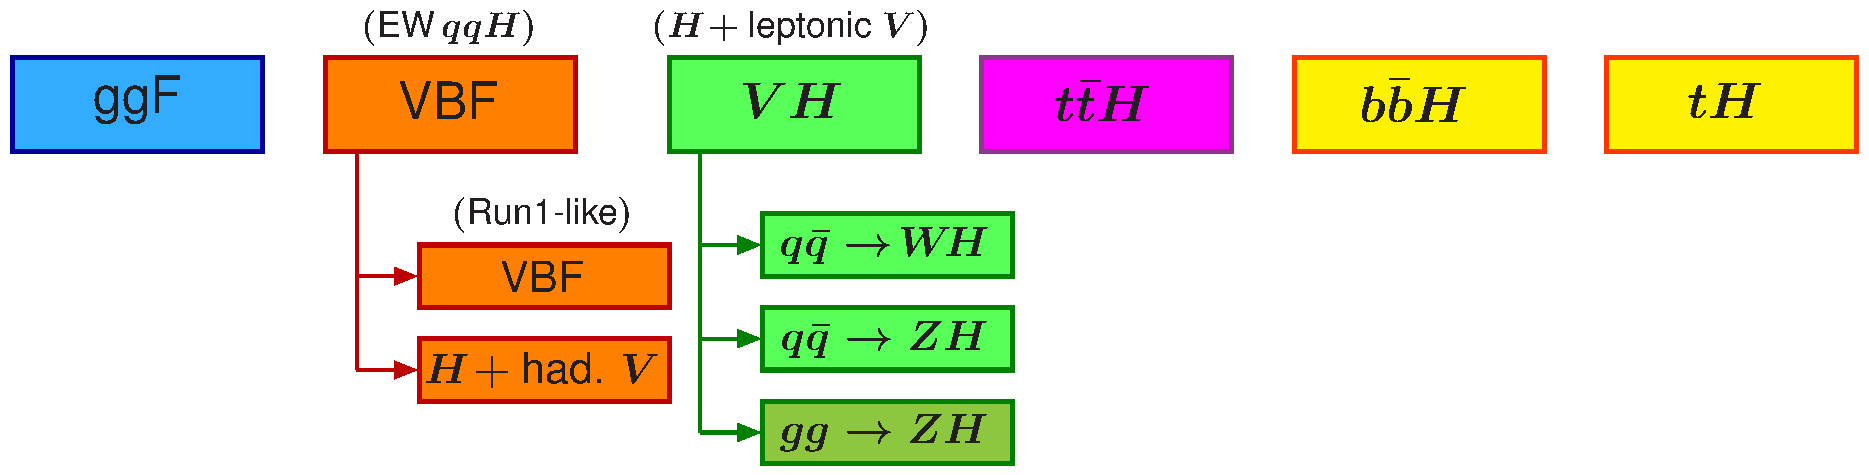
\includegraphics[width=\textwidth]{Figures/Theory/Higgs/STXS/simplifiedXS_stage0.pdf}
  \caption[Stage 0 Binning in the STXS]{Stage 0 binning in the STXS.}\label{fig:stxs_stage0}
\end{figure}

\begin{figure}[p]
  \centering
  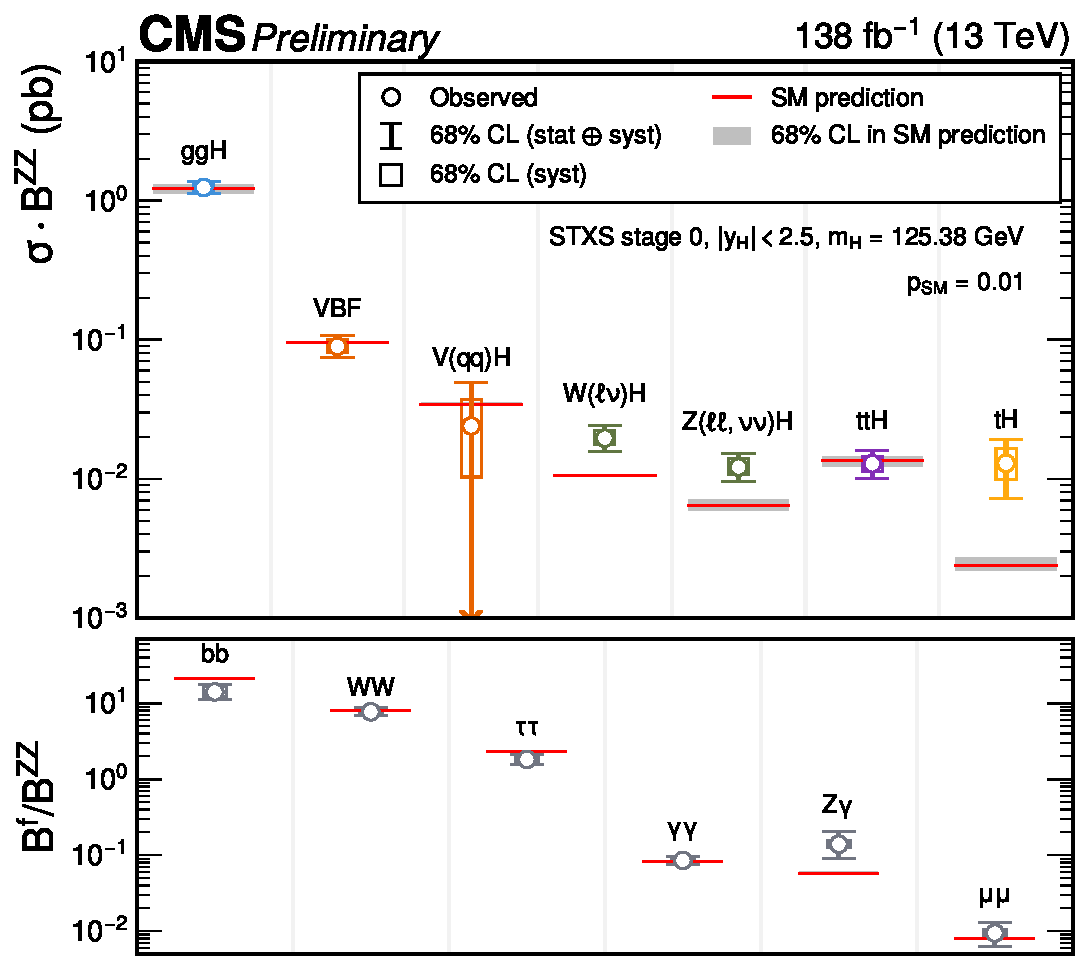
\includegraphics[width=0.8\textwidth]{Figures/Theory/Higgs/HIG-21-018-Figure_005-a.pdf}
  \caption[Measurements of the Stage 0 STXS]{STXS stage 0 cross sections and branching fraction ratios measured by the CMS experiment in a combination of Higgs boson decay channels in proton-proton collisions at $\sqrtS=13$\TeV corresponding to an integrated luminosity of 138\fbinv~\cite{CMS-PAS-HIG-21-018}. Theoretical uncertainties which affect the normalizations of the measured parameters are not included in the fit.}\label{fig:stage0_measurement}
\end{figure}

Additional information can be extracted by splitting the stage 0 bins further by e.g.\ the Higgs boson \pt, and this is where the later stages of the STXS come in. Schematics for the stage 1.2 binning are shown in \cref{fig:stxs_ggh,fig:stxs_vbf,fig:stxs_vh,fig:stxs_tth}. The variables used to split the bins, and the number of bins depends on the production mode. The stage 0 \ggH bin is split according to the Higgs boson transverse momentum, \ptH, the number of jets in the event, and in cases of $\geq 2$ jets, the invariant mass of the two leading jets, \mjj, and the transverse momentum of the Higgs boson and the two jets, \ptHjj. For $\ptH>200$\GeV, there is further splitting according to $\ptHj / \ptH$, where \ptHj is the transverse momentum of the Higgs boson and the leading jet. Excepting \ptHj, the stage 0 \qqH bin is split according to the same variables. The \VH bins are split by the transverse momentum of the vector boson, \ptV, and the number of jets in the event. The \ttH bin is split by \ptH only. Finally, the \bbH and \tH bins are not split further in stage 1.2 as there is limited experimental sensitivity to them.

\begin{figure}
  \centering
  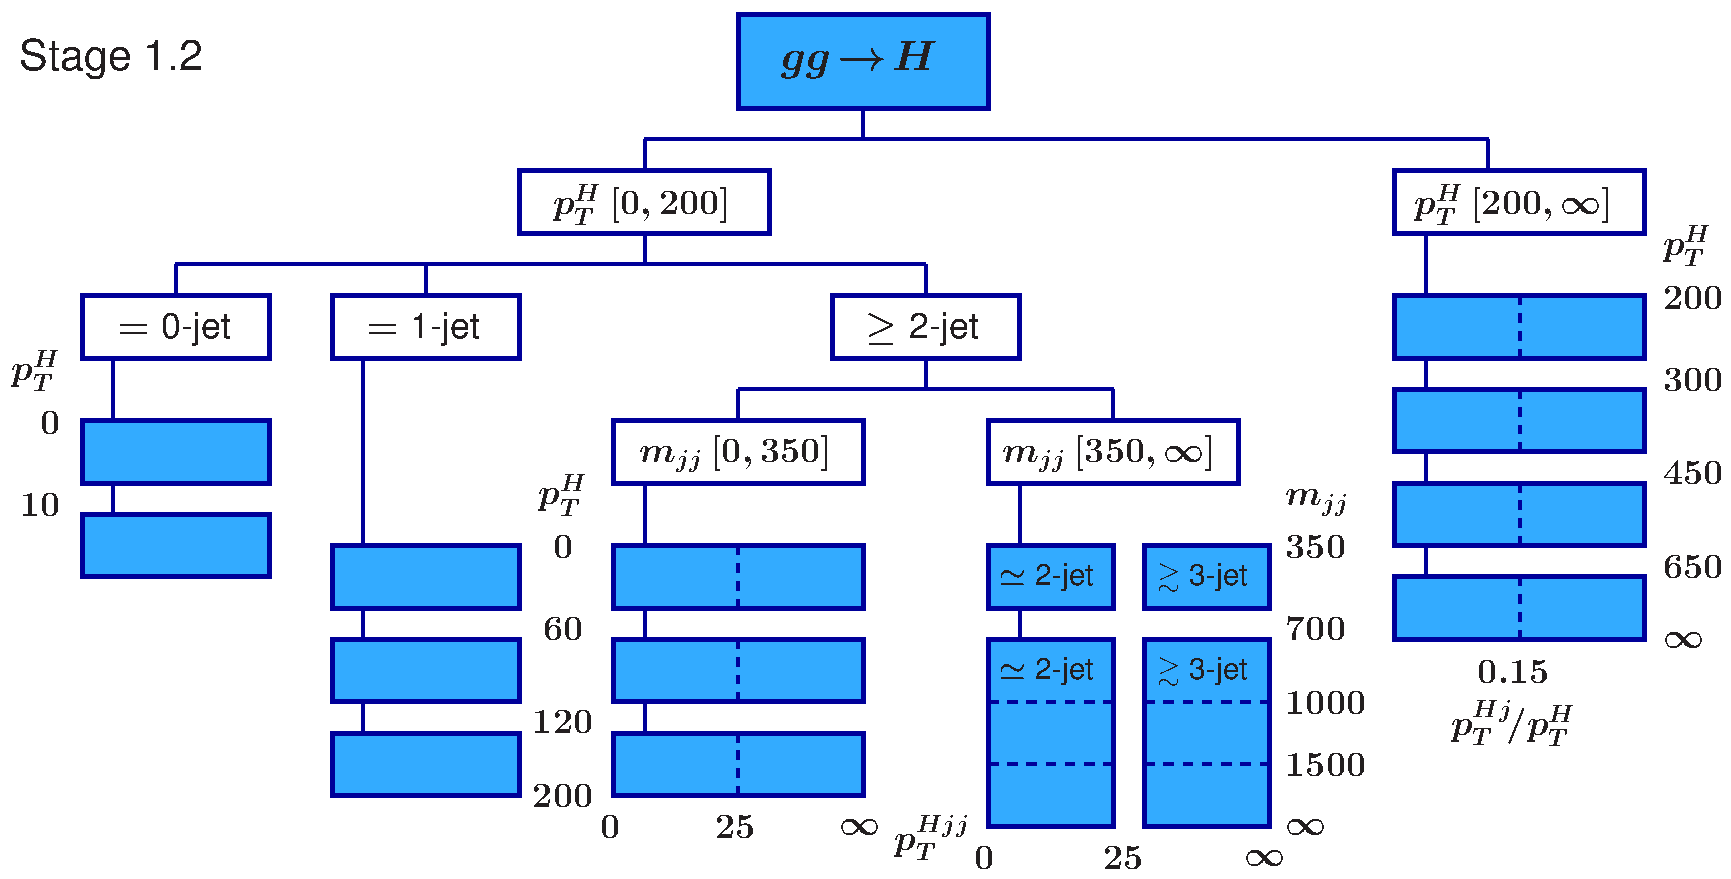
\includegraphics[width=\textwidth]{Figures/Theory/Higgs/STXS/simplifiedXS_ggF_1_2.pdf}
  \caption[Stage 1.2 \ggH Binning in the STXS]{Stage 1.2 binning for the \ggH production mode in the STXS.}\label{fig:stxs_ggh}
\end{figure}

\begin{figure}
  \centering
  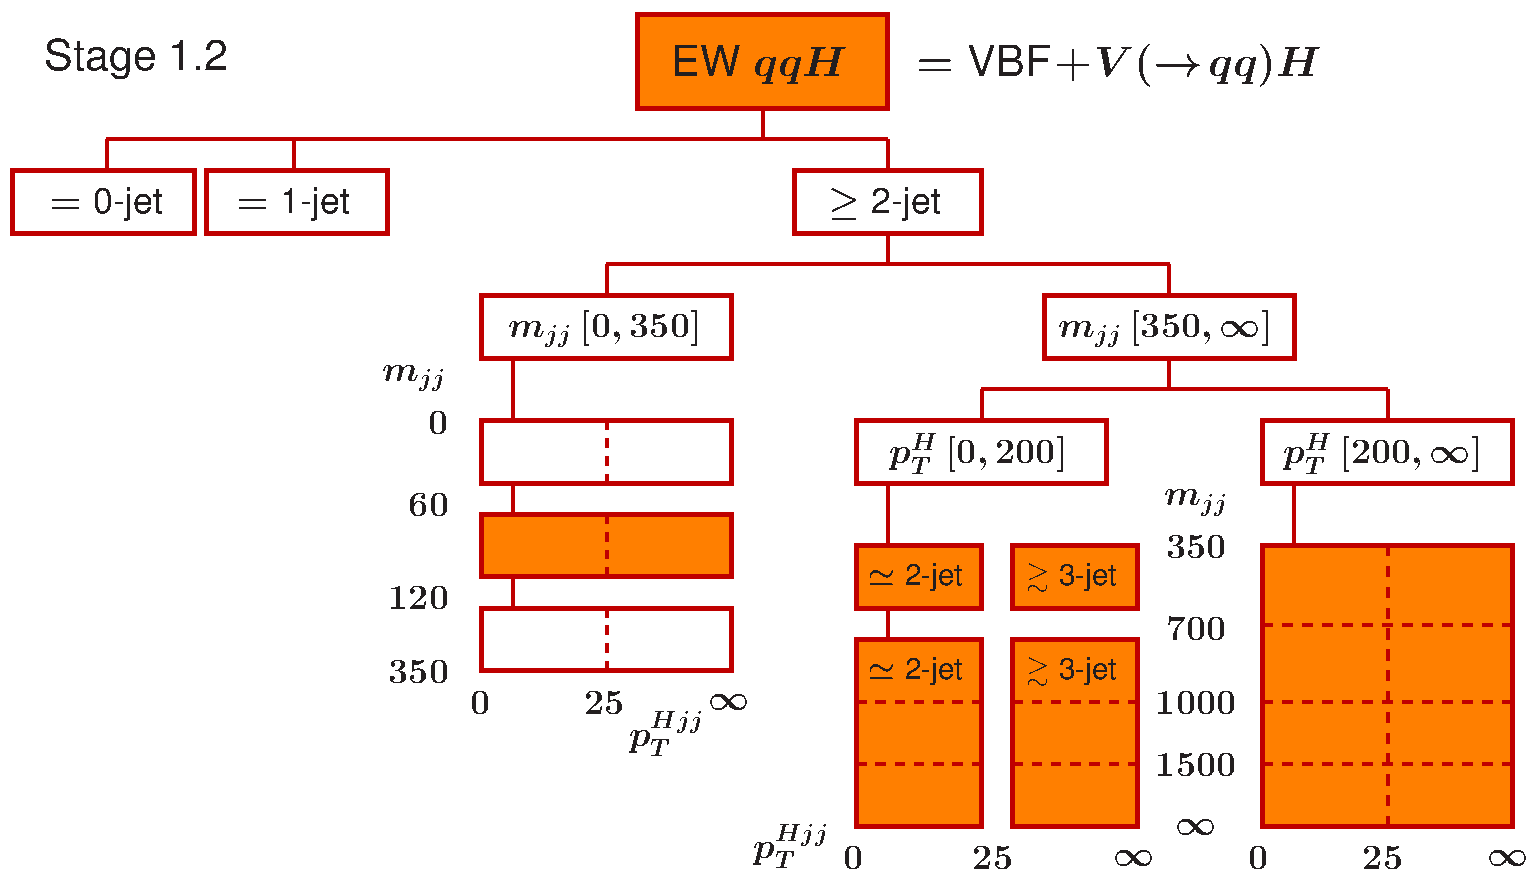
\includegraphics[width=0.8\textwidth]{Figures/Theory/Higgs/STXS/simplifiedXS_VBF_1_2.pdf}
  \caption[Stage 1.2 \VBF Binning in the STXS]{Stage 1.2 binning for the \qqH production mode in the STXS.}\label{fig:stxs_vbf}
\end{figure}

\begin{figure}
  \centering
  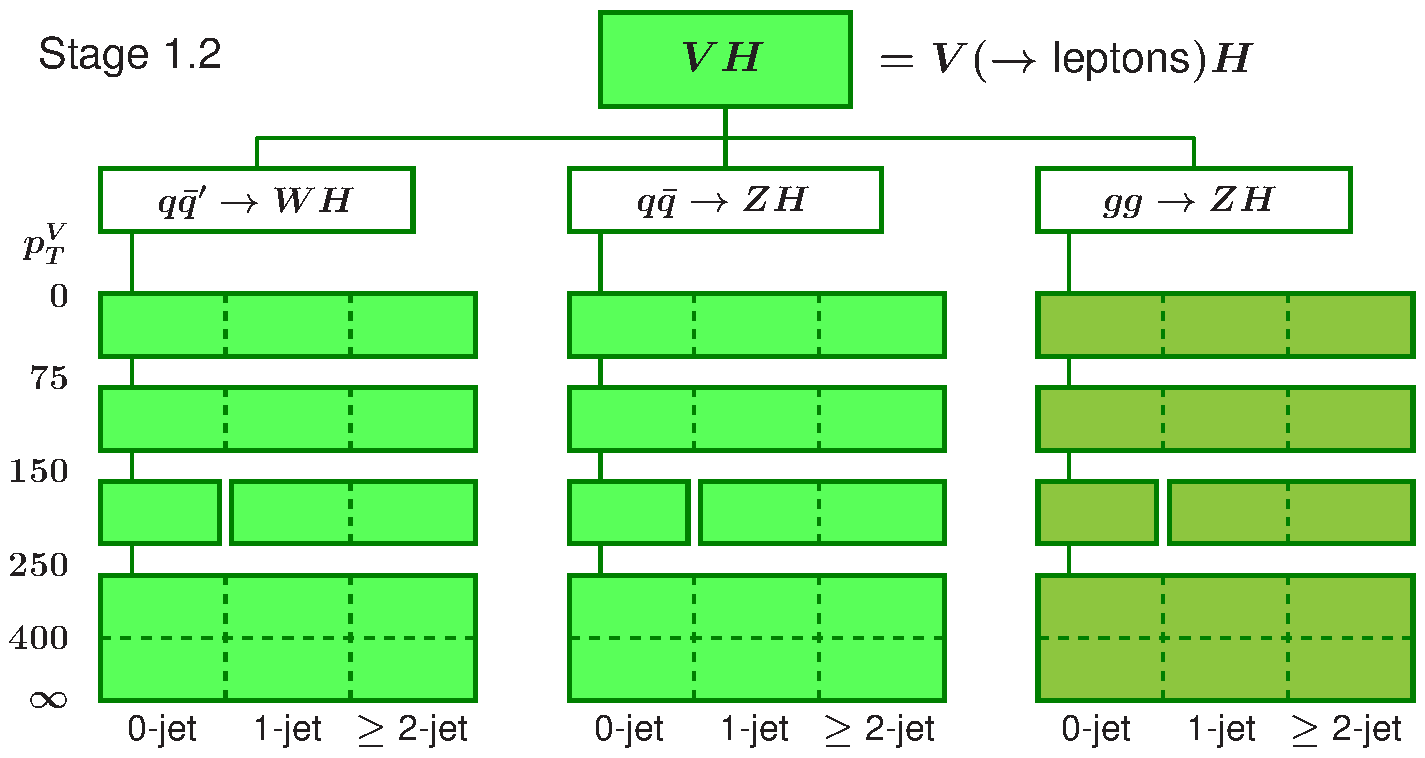
\includegraphics[width=0.8\textwidth]{Figures/Theory/Higgs/STXS/simplifiedXS_VH_1_2.pdf}
  \caption[Stage 1.2 \VH Binning in the STXS]{Stage 1.2 binning for the \VH leptonic production mode in the STXS.}\label{fig:stxs_vh}
\end{figure}

\begin{figure}
  \centering
  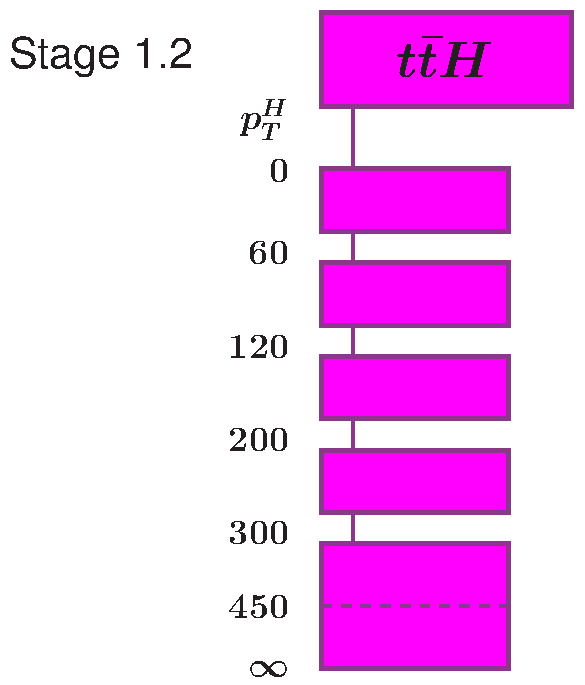
\includegraphics[width=0.3\textwidth]{Figures/Theory/Higgs/STXS/simplifiedXS_ttH_1_2.pdf}
  \caption[Stage 1.2 \ttH Binning in the STXS]{Stage 1.2 binning for the \ttH production mode in the STXS.}\label{fig:stxs_tth}
\end{figure}

The number of bins defined per production mode depends on the expected sensitivity, where \ggH, \qqH, \VH, and \ttH have 27, 24, 45, and 6 bins respectively where in \cref{fig:stxs_ggh,fig:stxs_vbf,fig:stxs_vh,fig:stxs_tth}, dashed lines indicate suggested places for bins to be merged. In the CMS combination~\cite{CMS-PAS-HIG-21-018}, a total of 32 bins were measured simultaneously: 13 for \ggH, 5 for \qqH, 4 for \WH leptonic, 4 for \ZH leptonic, 5 for \ttH, and a single bin for \tH. The results, in terms of $\sigma_i \cdot \BR^{\PZ\PZ}$ and $\BR^f / B^{\PZ\PZ}$, are shown in \cref{fig:stxs_stage1p2_results}. The compatibility with the SM is slightly better than the stage 0 results, with a p-value of 0.06. Now, in this stage 1.2 splitting, the \WH and \ZH disagreement can be identified as originating primarily by the $\ptV > 250$\GeV bins. 

\begin{figure}
  \centering
  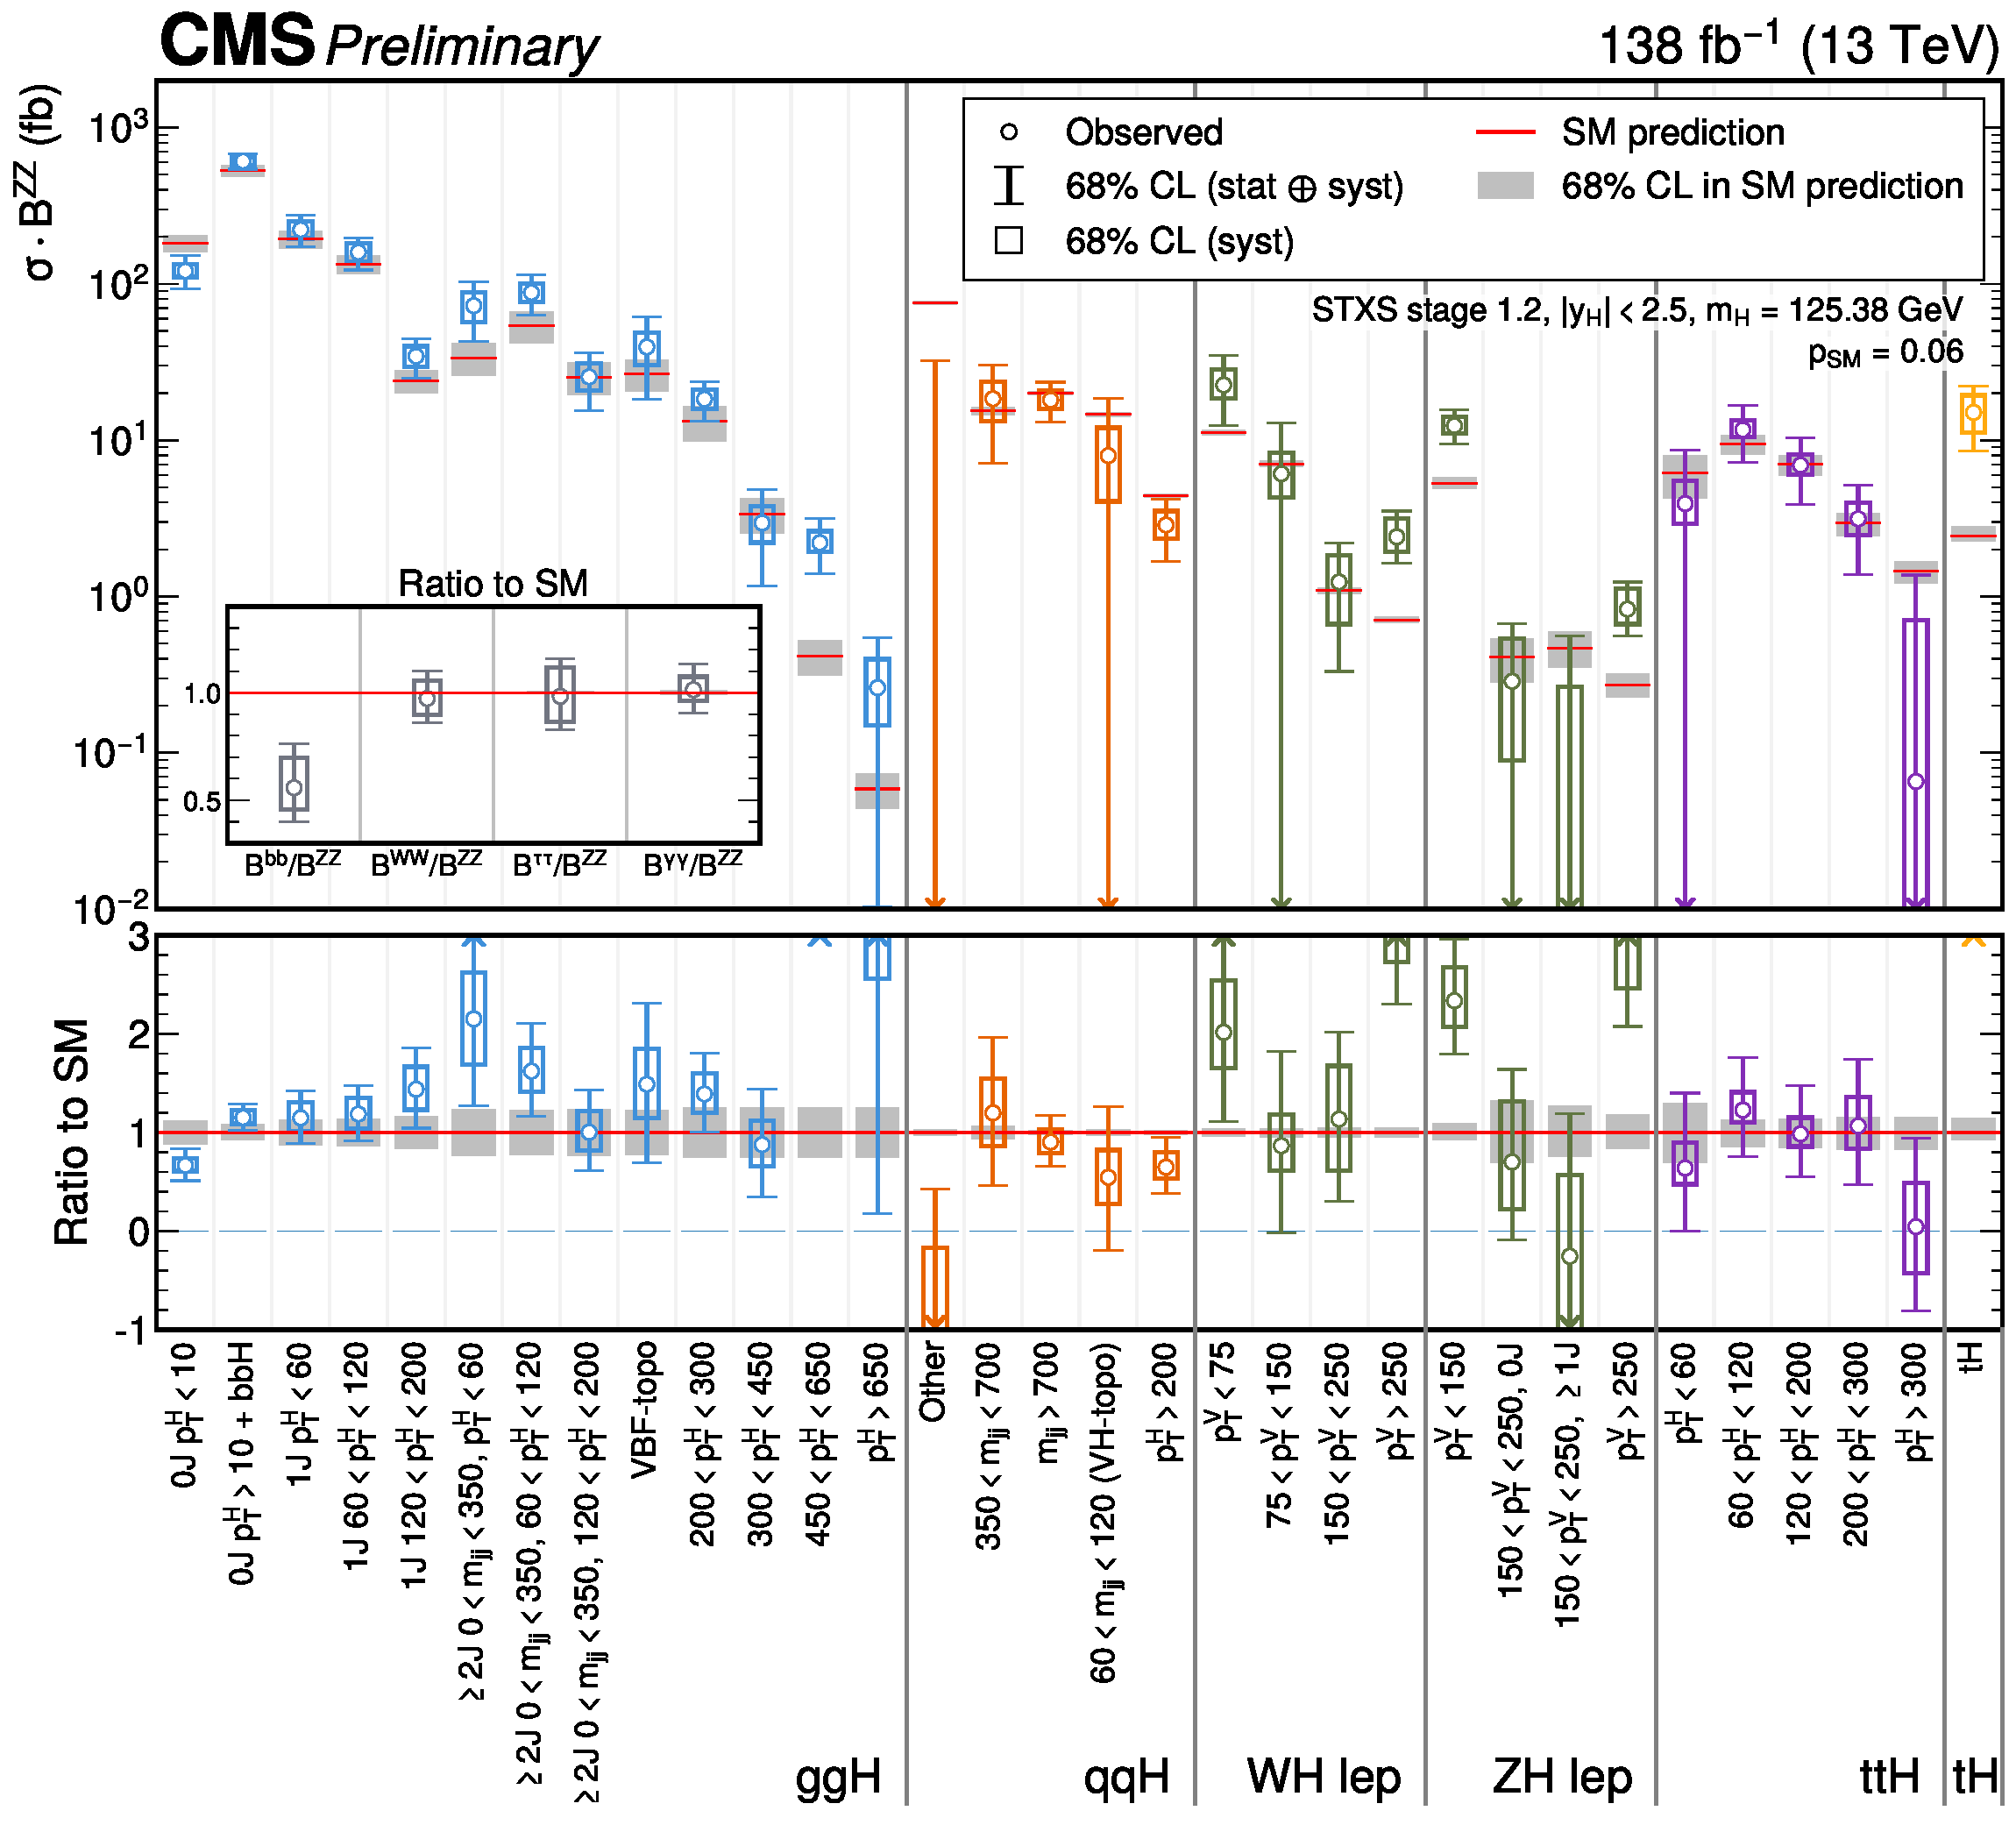
\includegraphics[width=\textwidth]{Figures/Theory/Higgs/HIG-21-018-Figure_006.pdf}
  \caption[Measurements of the Stage 1.2 STXS]{STXS stage 1.2 cross sections and branching fraction ratios measured by the CMS experiment in a combination of Higgs boson decay channels in proton-proton collisions at $\sqrtS=13$\TeV corresponding to an integrated luminosity of 138\fbinv~\cite{CMS-PAS-HIG-21-018}. Theoretical uncertainties which affect the normalizations of the measured parameters are not included in the fit. In cases where the best-fit values and/or 68\% CL intervals lie outside the range of the plot, their location (above or below) is indicated by arrows.}\label{fig:stxs_stage1p2_results}
\end{figure}

Finally, the results are also presented in terms of $\sigma_i \cdot \BR^f$ for every input decay channel as shown in \cref{fig:stxs_stage1p2_results_split}. Now, the origins of the disagreements in the cross sections can be identified from the individual decay channels and consistency checks can be performed. For example, enhancements in the high \ptV \WH leptonic bins are driven by the \Hbb, \HWW and \Htautau channels, and the excess for \tH is driven by the \Hgg channel which is the only channel with enough sensitivity to measure it separately from \ttH. 

A particular BSM theory can be confronted with these results by parameterizing the cross sections and branching fractions in terms of the theory's parameters, and then performing a fit to the data to place constraints on the theory parameters. This CMS combination does this with an Effective Field Theory (EFT), specifically the Standard Model EFT (SMEFT). The theoretical details underpinning this interpretation is discussed in \cref{sec:EFT} and the derivation of the SMEFT parameterization and the final results are discussed in \cref{chap:eft}.

\begin{landscape}
  \begin{figure}
    \centering
    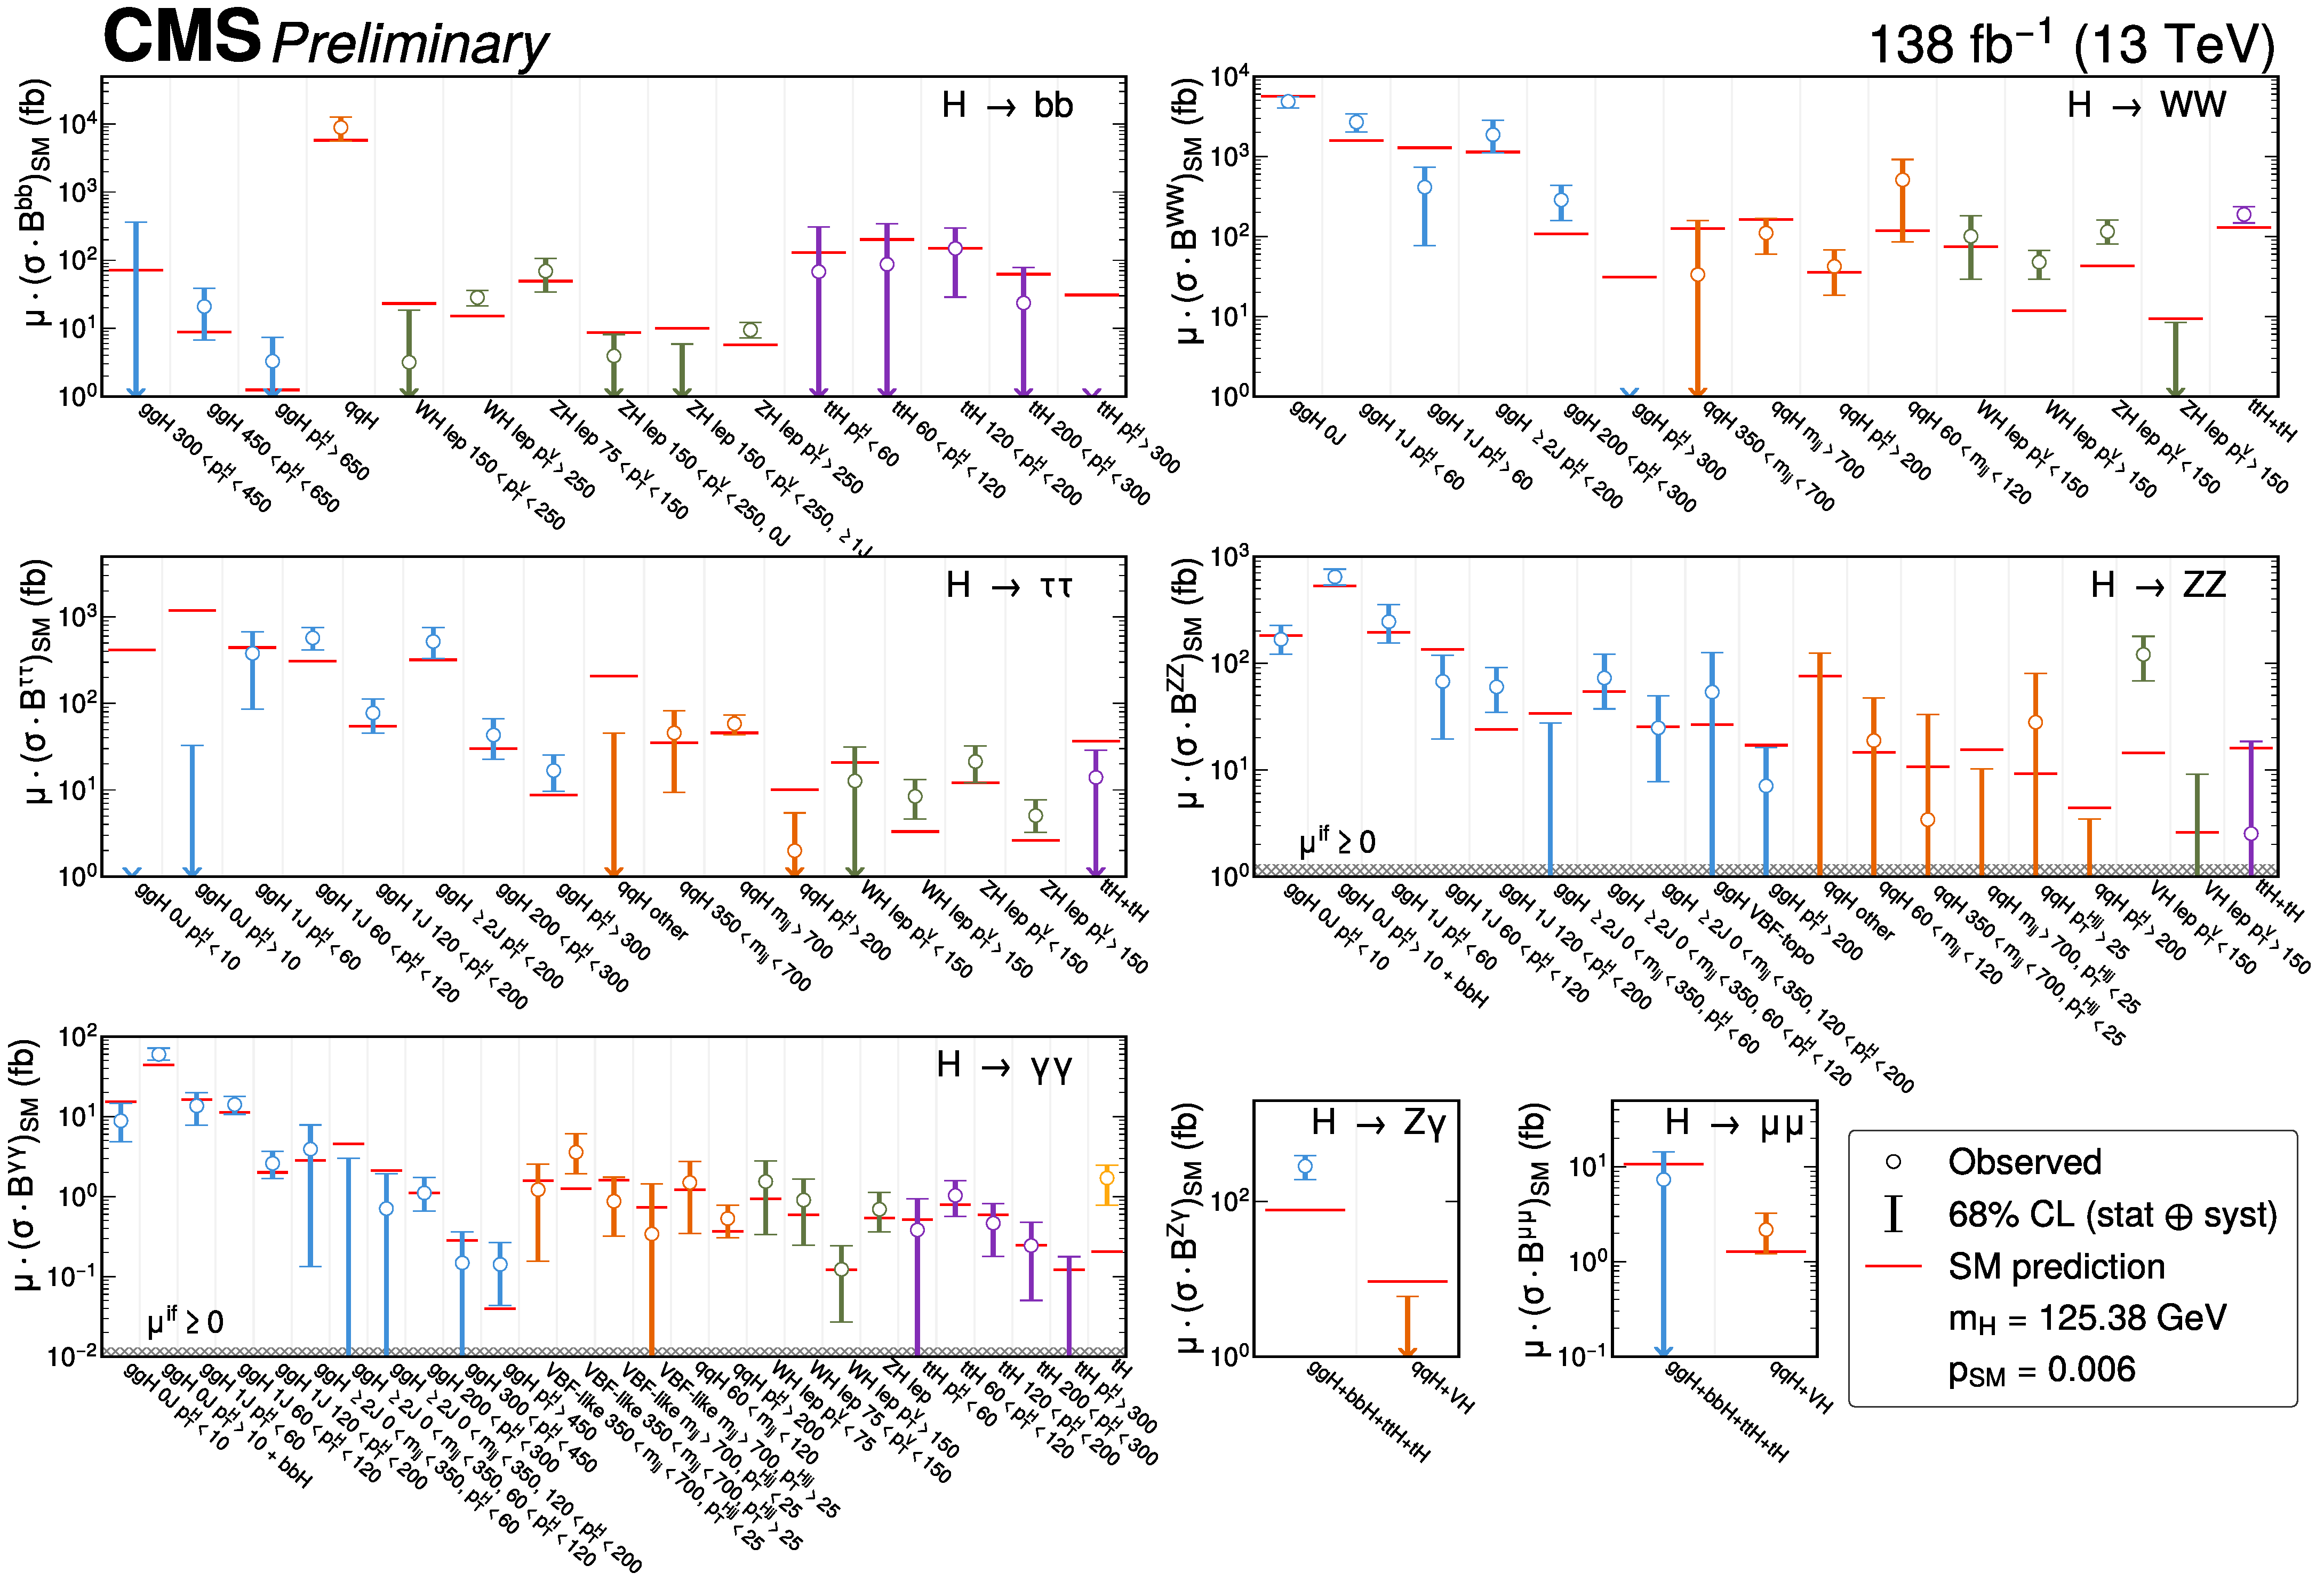
\includegraphics[width=0.9\pagewidth]{Figures/Theory/Higgs/HIG-21-018-Figure_008.pdf}
    \caption[Measurements of the Stage 1.2 STXS Split by Decay Channel]{STXS stage 1.2 cross section times branching fractions measured by the CMS experiment in a combination of Higgs boson decay channels in proton-proton collisions at $\sqrtS=13$\TeV corresponding to an integrated luminosity of 138\fbinv~\cite{CMS-PAS-HIG-21-018}. Theoretical uncertainties which affect the normalizations of the measured parameters are not included in the fit. In cases where the best-fit values and/or 68\% CL intervals lie outside the range of the plot, their location (above or below) is indicated by arrows. In the \Hgg and \HZZ decay channels, the results are constrained to be positive as indicated by the hatched grey lines.}\label{fig:stxs_stage1p2_results_split}
  \end{figure}
\end{landscape}
\section{Theories Beyond the Standard Model}\label{sec:bsm}
Theories beyond the Standard Model (BSM) can be used to explain anomalous observations such as dark matter~\cite{Clowe:2006eq}, and to solve theoretical problems like the hierarchy problem~\cite{Thomson:2013zua}. In this section, three theories (or families of theories) relevant to the experimental work presented in this thesis are discussed: Warped Extra Dimensions (WED), the Next-to-Minimal-Supersymmetric Standard Model (NMSSM), and Effective Field Theories (EFTs).

\subsection{Warped Extra Dimensions}\label{sec:wed}
In the Warped Extra Dimensions (WED) model~\cite{Randall:1999ee,Carvalho:2014lsg}, a five-dimensional geometry is proposed where a small spatial dimension is added to the traditional 4D spacetime. This theory alleviates the hierarchy problem and introduces two new \textit{gravity particles}: a spin-0 boson called the Radion which we denote \XZero, and a spin-2 boson called the Graviton which we denote \XTwo. Two theoretical scenarios are described in Ref.~\cite{Carvalho:2014lsg}, one where the SM particles are not allowed to propagate along the extra dimension and another where they are allowed, and these scenarios are referred to as the RS1 and Bulk scenarios respectively.

The decay channels and branching fractions for the Radion and Graviton are shown in \cref{fig:WED_BF}. In the Bulk scenario, the branching fraction to two SM Higgs bosons is about 30\% and about 10\% for the Radion and Graviton respectively for masses above 300\GeV. There are higher branching fractions to other decay channels such as \WW but more sensitive searches can be achieved with \HH if the right Higgs boson decay channels are chosen. One of the most competitive \HH decay channels is $b\bar{b}\gamma\gamma$ which has lower backgrounds and better mass resolution compared to $\PX \to \PW\PW$. 

Even better constraints can be achieved by performing searches with additional Higgs boson decay channels and then combining these searches, and this motivates the \XHH search in the $\gamma\gamma\tau\tau$ final state presented in \cref{chap:dihiggs}. In the RS1 scenario, the $\XTwo \to \PH\PH$ decay channel has a significantly lower branching fraction of around $\sim0.5\%$. Therefore, the search in \cref{chap:dihiggs} only considers the Bulk scenario. Production cross sections for the Radion and Graviton at $\sqrt{s}=13\TeV$ in the Bulk scenario are shown in \cref{fig:WED_xs} for particular values of $kl$, $\Lambda_R$ and $\tilde{k}$ which are free parameters of the theory and described in Ref.~\cite{Carvalho:2014lsg}. The dominant production mode for both the Radion and Graviton is gluon-gluon fusion.

\begin{figure}
  \centering
  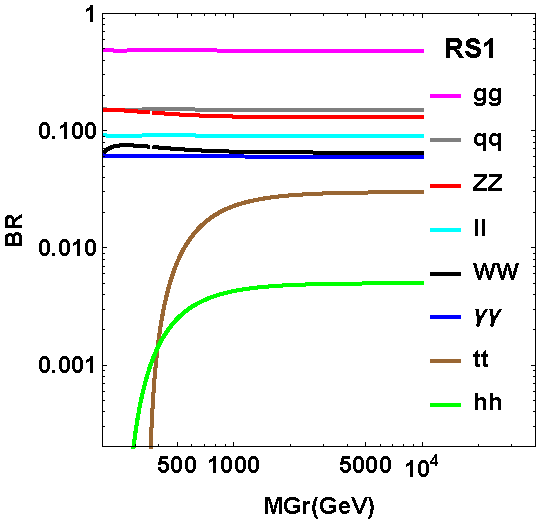
\includegraphics[width=0.49\textwidth]{Figures/Theory/WED/RSGravitonBRanal.pdf}
  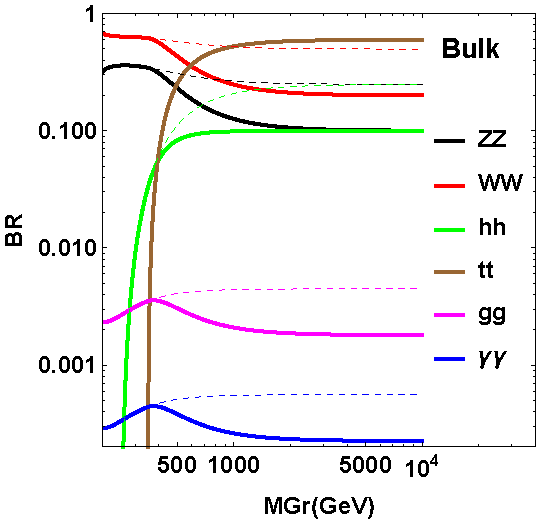
\includegraphics[width=0.49\textwidth]{Figures/Theory/WED/BulkGravitonBRanalWitTop.pdf}
  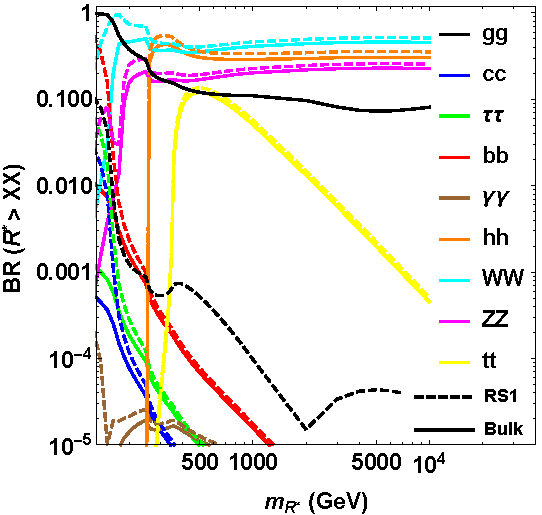
\includegraphics[width=0.49\textwidth]{Figures/Theory/WED/BR_eHDecay.pdf}
  \caption[Graviton and Radion Branching Fractions]{Branching fractions for the Graviton (top) and Radion (bottom) as functions of the particle masses. The RS1 and Bulk scenarios for the Graviton are shown in the top-left and top-right respectively whereas for the Radion, they are shown on the same plot and are differentiated by dashed and solid lines respectively. Figures are taken from Ref.~\cite{Carvalho:2014lsg}.}\label{fig:WED_BF}
\end{figure}

\begin{figure}
  \centering
  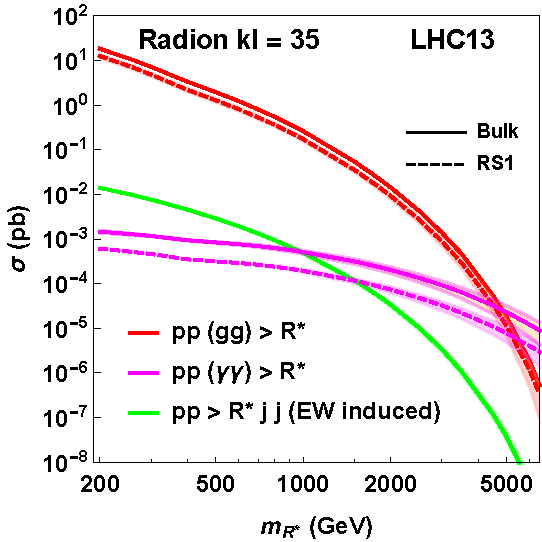
\includegraphics[width=0.48\textwidth]{Figures/Theory/WED/CX_RS_radion_13tev.pdf}
  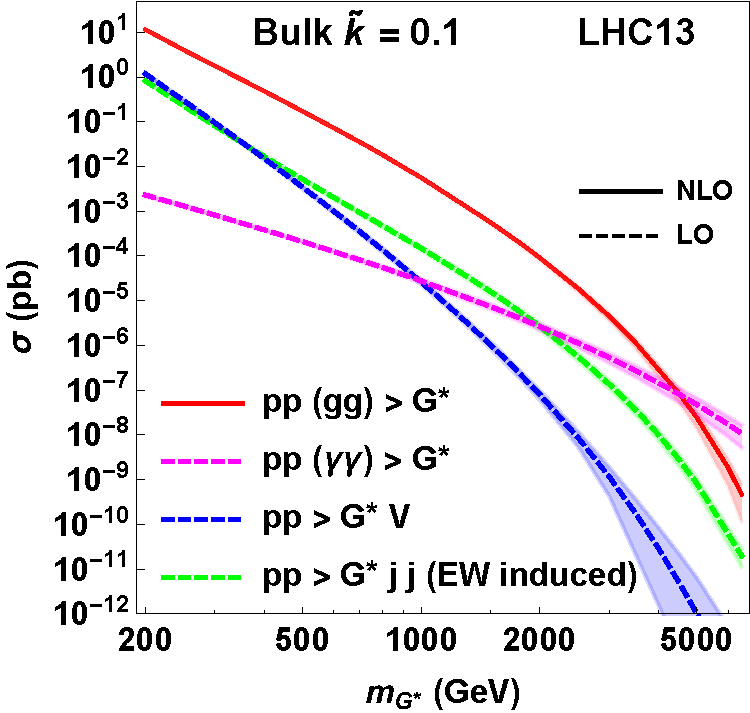
\includegraphics[width=0.49\textwidth]{Figures/Theory/WED/CX_bulk_13tev.pdf}
  \caption[Graviton and Radion Production Cross Sections]{Production cross sections at the LHC with $\sqrt{s}=13\TeV$ for the Radion ($R^*$) on the left, and the Graviton ($G^*$) on the right, shown as functions of the resonance masses. The Radion cross sections are shown for $kl=35$ and $\Lambda_R=3$\TeV and the Graviton cross sections are shown for $\tilde{k}=0.1$. Figures are taken from Ref.~\cite{Carvalho:2014lsg}.}\label{fig:WED_xs}
\end{figure}


\subsection{The Next-to-Minimal-Supersymmetric Standard Model}\label{sec:susy}
In supersymmetric theories, every SM particle has a \textit{superpartner} which differs in spin by $1/2$. In other words, every SM boson has a fermionic superpartner, and every SM fermion has a bosonic superpartner. Supersymmetric extensions of the SM are motivated by a solution to the hierarchy problem, an automatic unification of the running gauge couplings at a Grand Unified (GUT) scale $M_{\text{GUT}}$, and the introduction of a stable neutral particle which can be identified as a dark matter candidate~\cite{Ellwanger:2009dp}. 

In the Minimal Supersymmetric Standard Model (MSSM), there are two Higgs \SU{2}-doublets, $\Phi_1$ and $\Phi_2$, which lead to three neutral and two charged Higgs bosons~\cite{Fayet:1974pd,Fayet:1977yc}. An unattractive property of the MSSM is that the Lagrangian must contain a supersymmetric mass term for the Higgs doublets, which has to be of the order of the SUSY breaking scale, $M_{\text{SUSY}}$, for phenomenological reasons. Ideally, the electroweak scale generated by the Higgs vevs would depend only on $M_{\text{SUSY}}$, which would be the only remaining scale asking for an explanation as to why it is far below $M_{\text{GUT}}$ or the Planck scale $M_{\text{Planck}}$. This issue with the MSSM, denoted as the ``$\mu$-problem'', is rectified in the Next-to-Minimal Supersymmetric Standard Model (NMSSM)~\cite{Ellwanger:2009dp} and the solution requires the introduction of a singlet field, $S$. Models with this scalar structure are referred to as two-Higgs-doublet + singlet models (2HDM+S).

In 2DMH+S models, there are 3 CP-even and 2 CP-odd neutral scalars, and in the gauge eigenbasis these are denoted $H^{\text{SM}}$, $H^{\text{NSM}}$, $H^{\text{S}}$ and $A^{\text{NSM}}$, $A^{\text{S}}$ for the CP-even and CP-odd bosons respectively. The couplings of these states to SM particles are:
\begin{align*}
    H^{\text{SM}}(f_1,f_2,\mathrm{VV}) &= (g_{\text{SM}}, g_{\text{SM}}, g_{\text{SM}}), \\
    H^{\text{NSM}}(f_1,f_2,\mathrm{VV}) &= (g_{\text{SM}}/\tan{\beta}, -g_{\text{SM}}\tan{\beta}, 0), \\
    H^{\text{S}}(f_1,f_2,\mathrm{VV}) &= (0,0,0), \\
    A^{\text{NSM}}(f_1,f_2,\mathrm{VV}) &= (g_{\text{SM}}/\tan{\beta}, -g_{\text{SM}}\tan{\beta}, 0), \\
    A^{\text{S}}(f_1,f_2,\mathrm{VV}) &= (0,0,0)
\end{align*}
where $f_1$ ($f_2$) are SM fermions that couple to $\Phi_1$ ($\Phi_2$), $\mathrm{VV}$ corresponds to pairs of $\mathrm{W}$ or $\mathrm{Z}$ bosons, $g_{\text{SM}}$ is the coupling of a SM Higgs boson to such particles, and $\tan{\beta}$ is the ratio of vacuum expectation values: $\tan{\beta}=v_1/v_2$ where $v_1\equiv \langle \Phi_1 \rangle$ and  $v_2 \equiv \langle \Phi_2 \rangle$~\cite{Baum:2018zhf}.

The CP-even and CP-odd mass eigenstates obtained after mixing of gauge eigenstates are denoted $h_i=\{h_{125},H,h\}$ and $a_i=\{A,a\}$ respectively where $h_{125}$ is identified as the 125 GeV SM-like state observed at the LHC. The mass ordering is such that $m_H>m_h$ and $m_A>m_a$. In the alignment limit where $h_{125} = H^{\text{SM}}$, couplings for interactions involving $h_{125}h_{125}$ and one of the other scalars go to zero. On the other hand, couplings for $Hhh_{125}$ and $Aah_{125}$ are non-zero, which allows for so-called \textit{cascade decays}: $H\rightarrow h h_{125}$ and $A \rightarrow a h_{125}$. This motivates the \XYH search in \cref{chap:dihiggs} where \PX and \PY are new scalars, and \PH is the SM Higgs boson.

\subsubsection{$Y\rightarrow \gamma\gamma$ in the NMSSM at Low \mY}\label{sec:low_mass_in_NMSSM}

\begin{figure}
    \centering
    \inputtikz{Figures/Theory/SUSY/a_gamgam.tex}
    \caption[Feynman Diagram for a CP-Odd Higgs Boson Decaying to Two Photons Via a Chargino Loop]{Feynman diagram for the decay of the CP-odd Higgs boson, $a$, to two photons mediated by a chargino ($\chi^\pm$) loop.}\label{fig:a_gamgam}
   \end{figure}

If the lightest CP-odd Higgs in the mass basis, $a$, is very singlet-like, i.e.\ its main component is $A^S$, then its couplings to SM particles are heavily suppressed, and therefore, the typical hierarchy of Higgs decays: $bb, WW, \tau\tau, ZZ,\ldots$ becomes irrelevant. It is still possible for $a$ to decay to SM particles through loop interactions (see \cref{fig:a_gamgam}). The Higgs decay to two photons, which is suppressed in the SM, can now become the dominant decay mode for $a$, with a branching fraction up to 85\% depending on the theoretical scenario~\cite{King:2014xwa}. Since $a$ couples weakly to SM particles, its direct production, $pp \to a$ is also suppressed. The couplings of $a$ to BSM particles are however, not suppressed. Therefore, a search for $pp \rightarrow A \rightarrow a h_{125}$, where $a\to\gamma\gamma$, is uniquely placed to study this region of the NMSSM phase space. This motivates the inclusion of \Ygg in the \XYH search in \cref{chap:dihiggs}. 

In Ref.~\cite{Ellwanger:2022jtd}, maximally-allowed cross sections for this process are calculated given constraints from a set of relevant measurements. These cross sections are shown in \cref{fig:max_allowed_constraints}. If in the search for this process, we can set upper limits for the cross sections below the maximally-allowed, it means that our search will provide tighter constraints on the NMSSM than available at the time that Ref.~\cite{Ellwanger:2022jtd} was published (May 2022).

\begin{figure}[h]
    \centering
    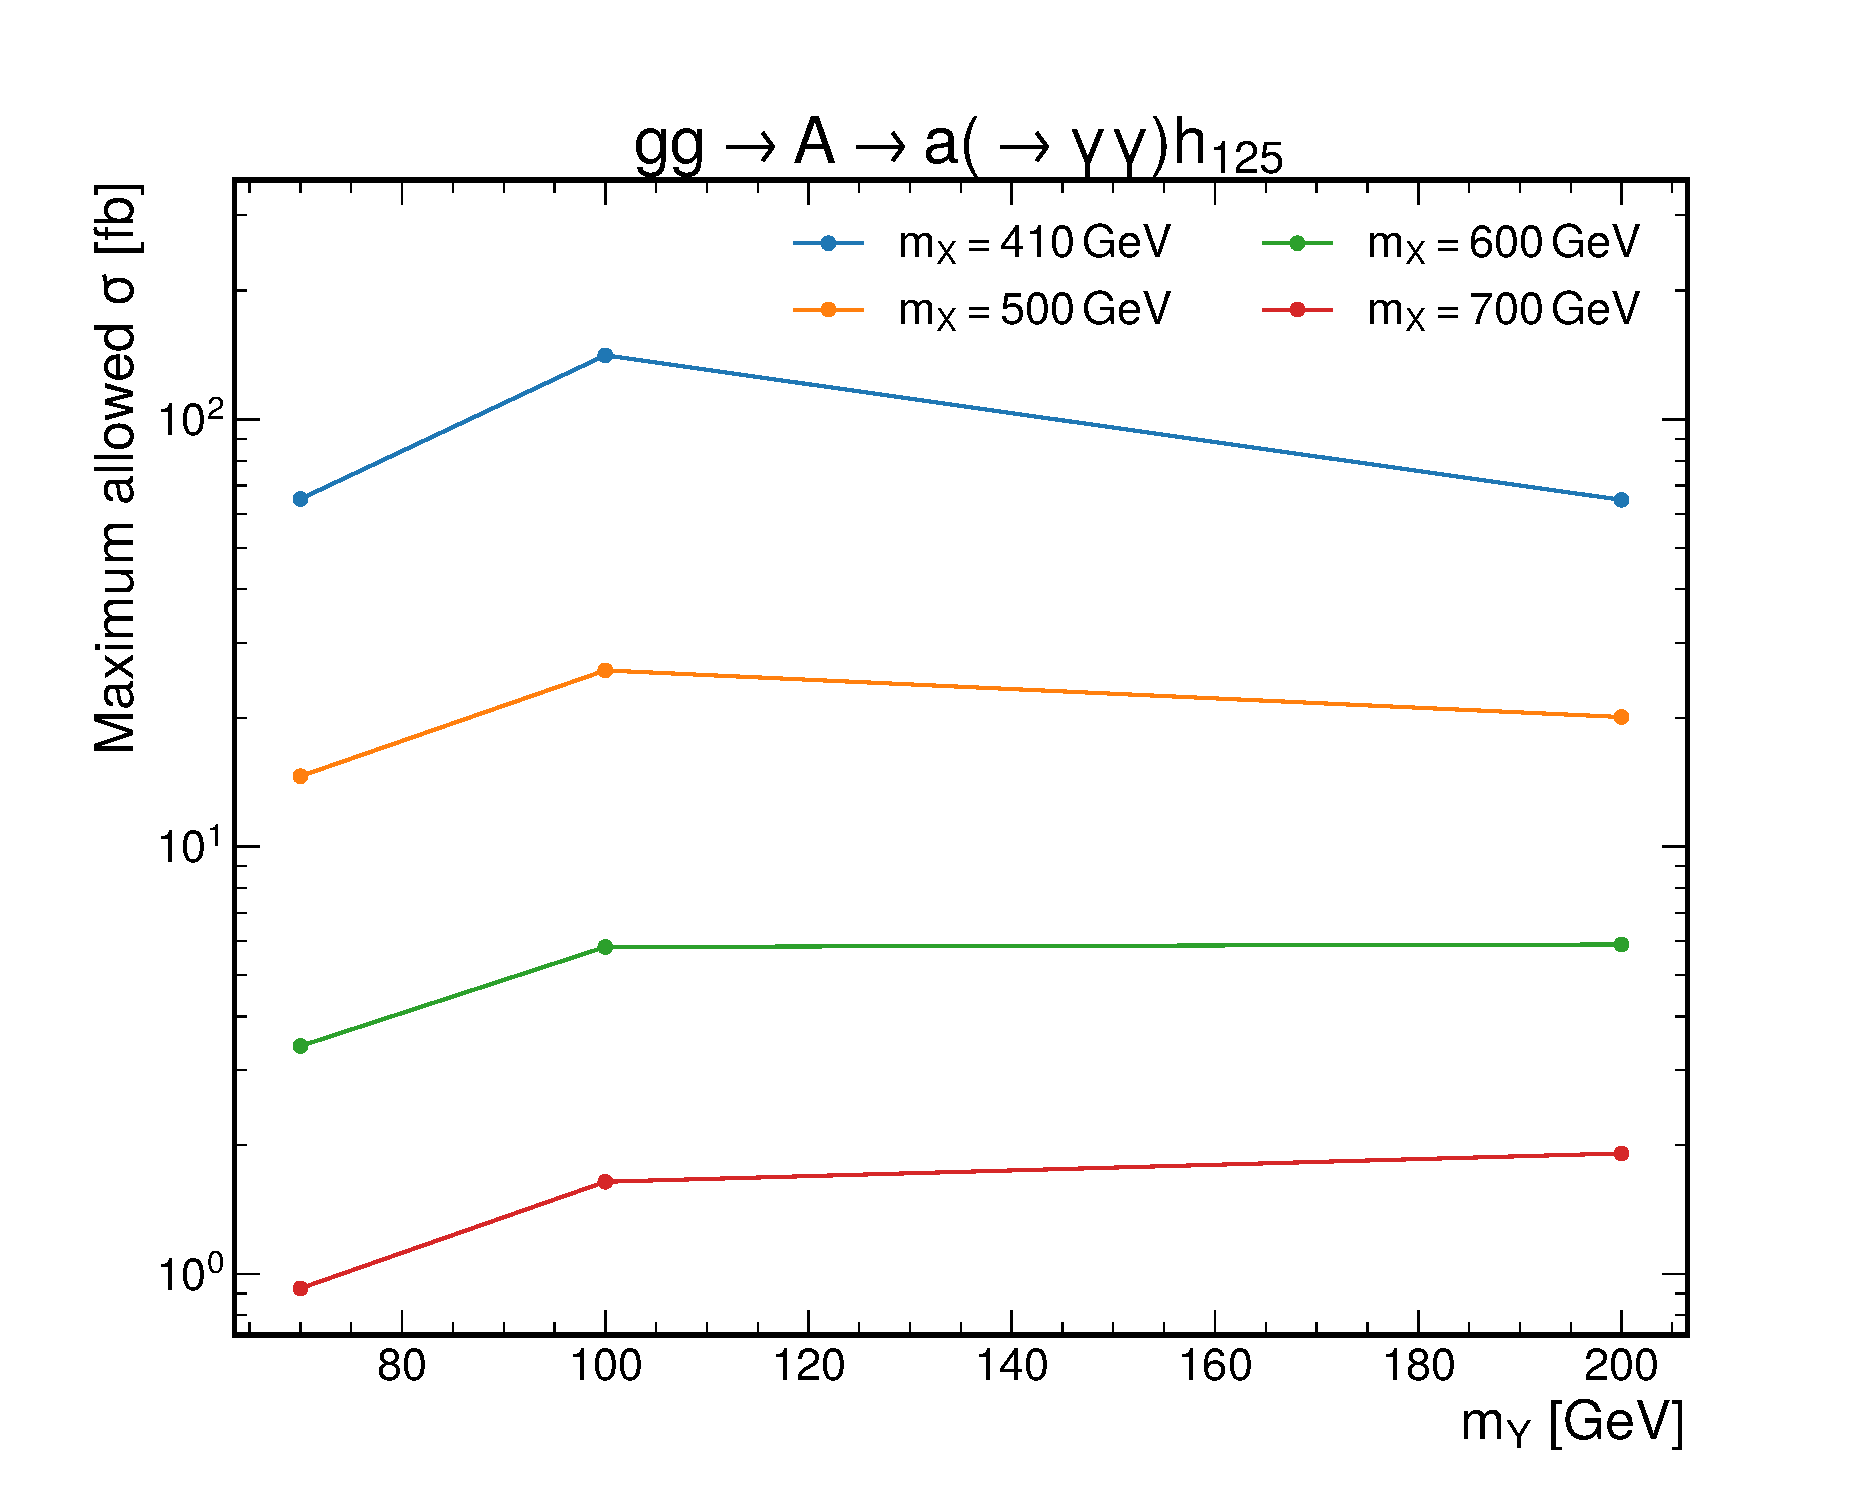
\includegraphics[width=0.7\textwidth]{Figures/Theory/SUSY/max_allowed_limits.pdf}
    \caption[Maximally-Allowed Cross Sections for $pp\rightarrow A \rightarrow H_{125}(\rightarrow\tau\tau)a(\rightarrow\gamma\gamma)$ in the NMSSM]{Maximally-allowed cross sections for $pp\rightarrow A \rightarrow h_{125}a(\rightarrow\gamma\gamma)$ in the NMSSM provided experimental constraints~\cite{Ellwanger:2022jtd}.}\label{fig:max_allowed_constraints}
\end{figure}
\newpage
\subsection{Effective Field Theory}\label{sec:EFT}
\subsubsection{Fermi Theory}

An effective field theory (EFT) is a low-energy approximation of another theory that is capable of making accurate predictions up to a particular energy scale. For example, the weak interaction can be approximated by an EFT called Fermi theory~\cite{Fermi:1934hr} which contains no description of the \PW or \PZ bosons. In the SM, muon decay is mediated by the exchange of a \PW boson but in Fermi theory, this is calculated using a four-point interaction (see \cref{fig:muon_decay_diagrams}). 

\begin{figure}
  \centering
  \inputtikz{Figures/Theory/EFT/muon_decay_sm.tex}
  \hspace{1cm}
  \inputtikz{Figures/Theory/EFT/muon_decay_fermi.tex}
  \caption[LO Feynman Diagrams for Muon Decay in the SM and in Fermi Theory]{LO Feynman diagrams for muon decay in the SM (left) and in Fermi theory (right).}\label{fig:muon_decay_diagrams}
\end{figure}

In the SM diagram, the mediating \PW boson, which is also referred to as a \textit{propagator}, introduces a term to the matrix element:
\begin{equation}
  \mathcal{M} = - i \frac{g_\mn - \frac{q_\mu q_\nu}{m_\PW^2}}{q^2 - m_\PW^2 + im_\PW \Gamma_\PW} \times \cdots
\end{equation}
where $q$ is the four-vector of the momentum transferred by the \PW boson, $\Gamma_\PW=2.09\GeV$ is the decay width of the \PW boson, and $g_\mn$ is the Minkowski metric.
In muon decay, $\sqrt{q^2} \ll m_\PW$ since $q^2 = m_\mu^2$ and given that $\Gamma_\PW \ll m_\PW$ as well, the propagator term is approximately:
\begin{equation}
  \frac{i g_\mn}{m_\PW^2}
\end{equation}
which, ignoring the vector indices, is a constant and can be absorbed into the coupling strength parameter of the Fermi theory, i.e.\ the theories are the same except for a factor of $1/m_\PW^2$ in the coupling strengths. The full calculation in Fermi theory predicts the decay width to be:
\begin{equation}
  \Gamma = \frac{G_F^2}{(\hbar c)^6}\frac{(m_\mu c^2)^5}{192 \pi^3}
\end{equation}
where $G_F$ is the \textit{Fermi constant} which characterizes the strength of the interaction. This can be related to the electroweak \SU{2} coupling, $g_2$, with:
\begin{equation}
  G_F = \frac{1}{4\sqrt{2}} \frac{g_2^2}{m_\PW^2}
\end{equation}
and therefore, a measurement of the muon decay width provides a relationship between the couplings of the weak interaction and the \PW boson mass. 

More generally, an interaction involving a propagator can be approximated by a point interaction if $q^2 \ll \Lambda^2$ where $\Lambda$ is the mass of the propagator. Then, measurements of interactions in that energy regime can be used to place constraints on the relationship between $g$ and $\Lambda$, where $g$ is a coupling parameter for these interactions. This extends to propagators outside the SM and therefore, EFT can be used to place constraints on new physics when using measurements at an energy scale much less than the mass of the new particle. 

\subsubsection{Standard Model Effective Field Theory}

The Standard Model Effective Field Theory (SMEFT) extends the SM Lagrangian by adding terms of higher dimension:
\begin{equation}
  \LSMEFT = \LSM + \frac{1}{\Lambda} \sum_i C_i^{(5)} O_i^{(5)} + \frac{1}{\Lambda^2} \sum_i C_i^{(6)} O_i^{(6)} + \cdots
  \label{eq:LSMEFT}
\end{equation}
where $O_i^{(d)}$ are dimension-$d$ terms called \textit{operators} that contain the SM fields and are invariant under the same gauge group as the SM, and $C_i^{(d)}$ are complex numbers called \textit{Wilson coefficients} that characterize the magnitude of each operator's contribution to \LSMEFT. Since \LSMEFT is a perturbative expansion, it requires that $C_i / \Lambda^d < \mathcal{O}(1)$ for all $C_i$.

We neglect all operators that violate lepton-number or baryon-number conservation and any operators that are dimension-7 or higher since they are suppressed by higher orders of $1 / \Lambda$. At dimension five, one operator remains which generates a Majorana mass term for neutrinos, and we also neglect this. The rest of this section will focus on the remaining dimension-6 terms which we denote by \Lsix.

We use a non-redundant basis for the operators called the Warsaw basis~\cite{Grzadkowski:2010es}. The basis definition is written in \cref{tab:Warsaw_basis}, using the following notation:
\begin{align}
  \tilde{X}^\mn &= \frac{1}{2} \epsilon^{\mn\rho\sigma} X_{\rho\sigma}, \quad &&H^\dag i \overleftrightarrow{D} H = H^\dag (i D_\mu H) - (i D_\mu H^\dag) H, \\
  \sigma^\mn &= \frac{i}{2} [\gamma^\mu, \gamma^\nu], &&H^\dag i \overleftrightarrow{D}^i H = H^\dag \sigma^i (i D_\mu H) - (i D_\mu H^\dag) \sigma^i H .
\end{align}

\clearpage
\thispagestyle{empty}
\begin{table}[h!]
  \begin{center}
  \small
  \hspace*{-2cm}
   \renewcommand{\arraystretch}{1.7}
   \begin{tabular}{|*3{>{$}c<{$}|>{$}p{4cm}<{$}|}}
  
   \toprule
   \multicolumn{2}{|c|}{$\mathcal{L}_6^{(1)}$ -- $X^3$} & 
    \multicolumn{2}{c|}{$\mathcal{L}_6^{(6)}$ -- $\psi^2 XH$}&
   \multicolumn{2}{c|}{$\mathcal{L}_6^{(8b)}$ -- $(\bar RR)(\bar RR)$}
   \\
  \midrule
  % c1
  Q_G & 
  f^{abc} G_\mu^{a\nu} G_\nu^{b\rho} G_\rho^{c\mu}  &
  % c6 
  Q_{eW} & 
  (\bar l_p \sigma^{\mu\nu} e_r) \sigma^i H W_{\mu\nu}^i &
  % 8b
  Q_{ee} & 
  (\bar e_p \gamma_\mu e_r)(\bar e_s \gamma^\mu e_t) 
  \\
  % c1
  Q_{\widetilde G} & 
  f^{abc} \widetilde G_\mu^{a\nu} G_\nu^{b\rho} G_\rho^{c\mu}  &
  % c6 
  Q_{eB} & 
  (\bar l_p \sigma^{\mu\nu} e_r) H B_{\mu\nu} &
  % 8b
  Q_{uu} & 
  (\bar u_p \gamma_\mu u_r)(\bar u_s \gamma^\mu u_t) 
  \\
  % c1
  Q_W & 
  \epsilon^{ijk} W_\mu^{i\nu} W_\nu^{j\rho} W_\rho^{k\mu} &
  % c6 
  Q_{uG} & 
  (\bar q_p \sigma^{\mu\nu} T^a u_r) \widetilde H \, G_{\mu\nu}^a &
  % 8b
  Q_{dd} & 
  (\bar d_p \gamma_\mu d_r)(\bar d_s \gamma^\mu d_t) 
  \\
  % c1
  Q_{\widetilde W}& 
  \epsilon^{ijk} \widetilde W_\mu^{i\nu} W_\nu^{j\rho} W_\rho^{k\mu} &
  % c6 
  Q_{uW} & 
  (\bar q_p \sigma^{\mu\nu} u_r) \sigma^i \widetilde H \, W_{\mu\nu}^i &
  % 8b
  Q_{eu} & 
  (\bar e_p \gamma_\mu e_r)(\bar u_s \gamma^\mu u_t) 
  \\\cline{1-2}
   \multicolumn{2}{|c|}{$\mathcal{L}_6^{(2)}$ -- $H^6$} &
  % c6 
  Q_{uB} & 
  (\bar q_p \sigma^{\mu\nu} u_r) \widetilde H \, B_{\mu\nu} &
  % 8b
  Q_{ed} & 
  (\bar e_p \gamma_\mu e_r)(\bar d_s\gamma^\mu d_t) 
  \\\cline{1-2}
  % c2
  Q_H & 
  (H^\dag H)^3 &
  % c6 
  Q_{dG} & 
  (\bar q_p \sigma^{\mu\nu} T^a d_r) H\, G_{\mu\nu}^a &
  % 8b
  Q_{ud}^{(1)} & 
  (\bar u_p \gamma_\mu u_r)(\bar d_s \gamma^\mu d_t) 
  \\
  \cline{1-2}
  \multicolumn{2}{|c|}{$\mathcal{L}_6^{(3)}$ -- $H^4 D^2$} &
  % c6 
  Q_{dW} & 
  (\bar q_p \sigma^{\mu\nu} d_r) \sigma^i H\, W_{\mu\nu}^i &
  % 8b
  Q_{ud}^{(8)} & 
  (\bar u_p \gamma_\mu T^a u_r)(\bar d_s \gamma^\mu T^a d_t) 
  \\\cline{1-2}
  % c3
  Q_{H\Box} & 
  (H^\dag H)\Box(H^\dag H) &
  % c6 
  Q_{dB} & 
  (\bar q_p \sigma^{\mu\nu} d_r) H\, B_{\mu\nu} &
  % c8b
  &
  \\
  % c3
  Q_{H D} & 
  \ \left(D^\mu H^\dag  H\right) \left(H^\dag D_\mu H\right) &
  %c6
  &&
  % c8b
  &
  \\\midrule
   \multicolumn{2}{|c|}{$\mathcal{L}_6^{(4)}$ -- $X^2H^2$}& 
   \multicolumn{2}{c|}{$\mathcal{L}_6^{(7)}$ -- $\psi^2H^2 D$}& 
   \multicolumn{2}{c|}{$\mathcal{L}_6^{(8c)}$ -- $(\bar LL)(\bar RR)$}
  \\\midrule
  % c4
  Q_{H G}  & 
  H^\dag H\, G^a_{\mu\nu} G^{a\mu\nu} &
  % c7
  Q_{H l}^{(1)} & 
  (H^\dag i\overleftrightarrow{D}_\mu H)(\bar l_p \gamma^\mu l_r)&
  % 8c
  Q_{le} & 
  (\bar l_p \gamma_\mu l_r)(\bar e_s \gamma^\mu e_t)
  \\
  % c4
  Q_{H\widetilde G} & 
  H^\dag H\, \widetilde G^a_{\mu\nu} G^{a\mu\nu} &
  % c7
  Q_{H l}^{(3)} & 
  (H^\dag i\overleftrightarrow{D}^i_\mu H)(\bar l_p \sigma^i \gamma^\mu l_r)&
  % 8c
  Q_{lu} & 
  (\bar l_p \gamma_\mu l_r)(\bar u_s \gamma^\mu u_t) 
  \\
  % c4
  Q_{H W} & 
  H^\dag H\, W^i_{\mu\nu} W^{I\mu\nu} &
  % c7
  Q_{H e} & 
  (H^\dag i\overleftrightarrow{D}_\mu H)(\bar e_p \gamma^\mu e_r)&
  % 8c
  Q_{ld} & 
  (\bar l_p \gamma_\mu l_r)(\bar d_s \gamma^\mu d_t) 
  \\
  % c4
  Q_{H\widetilde W} & 
  H^\dag H\, \widetilde W^i_{\mu\nu} W^{i\mu\nu} &
  % c7
  Q_{H q}^{(1)} & 
  (H^\dag i\overleftrightarrow{D}_\mu H)(\bar q_p \gamma^\mu q_r)&
  % 8c
  Q_{qe} & 
  (\bar q_p \gamma_\mu q_r)(\bar e_s \gamma^\mu e_t)
  \\
  % c4
  Q_{H B} &  H^\dag H\, B_{\mu\nu} B^{\mu\nu} &
  % c7
  Q_{H q}^{(3)} & 
  (H^\dag i\overleftrightarrow{D}^i_\mu H)(\bar q_p \sigma^i \gamma^\mu q_r)&
  % 8c
  Q_{qu}^{(1)} & 
  (\bar q_p \gamma_\mu q_r)(\bar u_s \gamma^\mu u_t)
  \\
  % c4
  Q_{H\widetilde B} & 
  H^\dag H\, \widetilde B_{\mu\nu} B^{\mu\nu} &
  % c7
  Q_{H u} & 
  (H^\dag i\overleftrightarrow{D}_\mu H)(\bar u_p \gamma^\mu u_r)&
  % 8c
  Q_{qu}^{(8)} & 
  (\bar q_p \gamma_\mu T^a q_r)(\bar u_s \gamma^\mu T^a u_t) 
  \\
  % c4
  Q_{H WB} & 
   H^\dag \sigma^i H\, W^i_{\mu\nu} B^{\mu\nu} &
  % c7
  Q_{H d} & 
  (H^\dag i\overleftrightarrow{D}_\mu H)(\bar d_p \gamma^\mu d_r)&
  % 8c
  Q_{qd}^{(1)} & 
  (\bar q_p \gamma_\mu q_r)(\bar d_s \gamma^\mu d_t) 
  \\
  % c4
  Q_{H\widetilde W B} & 
  H^\dag \sigma^i H\, \widetilde W^i_{\mu\nu} B^{\mu\nu} &
  % c7
  Q_{H u d}+\hc & 
  i(\widetilde H ^\dag D_\mu H)(\bar u_p \gamma^\mu d_r)&
  % 8c
  Q_{qd}^{(8)} & 
  (\bar q_p \gamma_\mu T^a q_r)(\bar d_s \gamma^\mu T^a d_t)
  \\
  \midrule
   \multicolumn{2}{|c|}{$\mathcal{L}_6^{(5)}$ -- $\psi^2 H^3$} &
   \multicolumn{2}{c|}{$\mathcal{L}_6^{(8a)}$ -- $(\bar LL)(\bar LL)$}&
   \multicolumn{2}{c|}{$\mathcal{L}_6^{(8d)}$ -- $(\bar LR)(\bar RL)$, $(\bar LR)(\bar LR)$} 
   \\\midrule
  % c5
  Q_{eH} & 
  (H^\dag H)(\bar l_p e_r H) &
  % 8a 
  Q_{ll}  & 
  (\bar l_p \gamma_\mu l_r)(\bar l_s \gamma^\mu l_t)&
  % 8d
  Q_{ledq} & 
  (\bar l_p^j e_r)(\bar d_s q_{tj})
  \\
  % c5
  Q_{uH}  &
  (H^\dag H)(\bar q_p u_r \widetilde H )&
  % 8a
  Q_{qq}^{(1)} & 
  (\bar q_p \gamma_\mu q_r)(\bar q_s \gamma^\mu q_t) &
  % 8d 
  Q_{quqd}^{(1)} & 
  (\bar q_p^j u_r) \epsilon_{jk} (\bar q_s^k d_t) 
  \\
  % c5
  Q_{dH}  & 
  (H^\dag H)(\bar q_p d_r H)&
  % 8a 
  Q_{qq}^{(3)} & 
  (\bar q_p \gamma_\mu \sigma^i q_r)(\bar q_s \gamma^\mu \sigma^i q_t) &
  % 8d
  Q_{quqd}^{(8)} & 
  (\bar q_p^j T^a u_r) \epsilon_{jk} (\bar q_s^k T^a d_t) 
  \\
  % c5
  &&
  % 8a 
  Q_{lq}^{(1)} & 
  (\bar l_p \gamma_\mu l_r)(\bar q_s \gamma^\mu q_t)&
  % 8d
  Q_{lequ}^{(1)} & 
  (\bar l_p^j e_r) \epsilon_{jk} (\bar q_s^k u_t) 
  \\
  % c5
  &&
  % 8a 
  Q_{lq}^{(3)} & 
  (\bar l_p \gamma_\mu \sigma^i l_r)(\bar q_s \gamma^\mu \sigma^i q_t) &
  % 8d
  Q_{lequ}^{(3)} & 
  (\bar l_p^j \sigma_{\mu\nu} e_r) \epsilon_{jk} (\bar q_s^k \sigma^{\mu\nu} u_t) 
  \\\bottomrule
  \end{tabular}
  % }
  \end{center}
  \caption[Warsaw Basis of Operators]{$\mathcal{L}_6$ operators in the Warsaw basis~\cite{Grzadkowski:2010es}, categorized into eight classes $\mathcal{L}_6^{(n)}$ as in~\cite{Alonso:2013hga}. Only baryon number-conserving invariants are retained. The flavor indices $p,r,s,t$ are suppressed in the operators' labels.}\label{tab:Warsaw_basis}
  \end{table}

In \cref{tab:Warsaw_basis}, there are 59 independent operators and naively, one might expect therefore, that there are only 59 Wilson coefficients that need to be measured to specify the theory. However, some operators carry flavour indices of which all combinations need to be summed over:
\begin{equation}
  \Lsix = \frac{1}{\Lambda^2} \sum_i \sum^3_{p,r=1} C_{i,pr} Q_{i,pr} + \cdots
  \label{eq:smeft_flavour_combinations}
\end{equation}
and this leads to a higher number of Wilson coefficients. In total, there are 2599 free parameters in \Lsix, counting real and imaginary components of the Wilson coefficients separately. It is not currently possible to experimentally constrain all of these parameters simultaneously and nor will it be in the short-term future. Therefore, we use flavour assumptions to reduce the number of free parameters to a more reasonable level.

\subsubsection{Flavour Assumptions}
The most restrictive flavour assumption we can make is the symmetry of the kinetic terms: $\U{3}^5 = \U{3}_q \times \U{3}_u \times \U{3}_d \times \U{3}_l \times\U{3}_e$, where each field is assigned to a three-component representation of the associated group. In this assumption, the terms in \cref{eq:smeft_flavour_combinations} become:
\begin{equation}
  \mathcal{L}_6 = \frac{1}{\Lambda^2} \sum_i \sum^3_{p,r=1} C_i X_{i,pr} Q_{i,pr} + \cdots
  \label{eq:smeft_flavour_combinations_u35}
\end{equation}
where the flavour structure of each operator is factored out into $X_{i,pr}$ leaving a single Wilson coefficient per operator. Under the $\U{3}^5$ flavour assumption, there are a total of 85 free parameters.

If a set of measurements can distinguish an operator's effect on one flavour of fermion from another, e.g.\ by combining measurements of top-quark production and light-jet production, then we need not be so restrictive with our flavour assumption. A less restrictive option compared to $\U{3}^5$ is the so-called \topUtl assumption~\cite{Brivio:2020onw} where the quarks of the first two generations and quarks of the 3rd are described by independent fields, denoted $(q_p, u_p, d_p)$ and $(Q, t, b)$ respectively. The fermionic operators in this basis are provided in \cref{tab:topU3l_basis}. A $\U{2}^3 = \U{2}_q \times \U{2}_u \times \U{2}_d$ symmetry is imposed in the quark sector and paired with a $\U{3}^2 = \U{3}_l \times \U{3}_e$ symmetry in the lepton sector. With this flavour assumption, an operator can contribute differently to processes involving the first two generations from processes involving the third. Therefore, we can probe new physics effects that have a hierarchical structure in the quark sector. In the SMEFT interpretation described in \cref{chap:eft}, the \topUtl assumption is used.

\clearpage
\thispagestyle{empty}
\begin{table}
\vspace*{-2cm}
\small
\hspace*{-2.3cm}
\scalebox{.76}{
\renewcommand{\arraystretch}{1.6}\begin{tabular}{|*4{>{$}c<{$}|>{$}l<{$}|}}
\toprule

\multicolumn{8}{|c|}{$\mathcal{L}_6^{(5)} - \psi^2 H^3$}
\\\midrule
Q_{uH}& (H^\dag H) (\bar q \, Y_u^\dag \, u \tilde H) 
& 
Q_{dH}& (H^\dag H) (\bar q\, Y_d^\dag\, d H)
& 
Q_{eH}& (H^\dag H) (\bar l_p e_r H)
&  & 
\\
Q_{tH}& (H^\dag H) (\bar Q  \tilde Ht)
&
Q_{bH}& (H^\dag H) (\bar Q H b)
& &
& &
\\\midrule

\multicolumn{8}{|c|}{$\mathcal{L}_6^{(6)} - \psi^2 X H$}
\\\midrule
Q_{eW}& (\bar l_p \sigma^{\mu\nu} e_r) \sigma^i H W_{\mu\nu}^i
&
Q_{uW}& (\bar q\, Y_u^\dag\, \sigma^{\mu\nu} u) \sigma^i \tilde H W_{\mu\nu}^i
&
Q_{uB}& (\bar q\, Y_u^\dag\, \sigma^{\mu\nu} u) \tilde H B_{\mu\nu}
&
Q_{uG}& (\bar q\, Y_u^\dag\, \sigma^{\mu\nu} T^a u) \tilde H G_{\mu\nu}^a
\\
Q_{eB}& (\bar l_p \sigma^{\mu\nu} e_r) H B_{\mu\nu}
&
Q_{tW}& (\bar Q \sigma^{\mu\nu} t) \sigma^i \tilde H W_{\mu\nu}^i
&
Q_{tB}& (\bar Q \sigma^{\mu\nu} t)  \tilde H B_{\mu\nu}
&
Q_{tG}& (\bar Q \sigma^{\mu\nu} T^a t) \tilde H G_{\mu\nu}^a
\\
Q_{dW}& (\bar q\, Y_d^\dag\, \sigma^{\mu\nu} d) \sigma^i H W_{\mu\nu}^i
&
Q_{dB}& (\bar q\, Y_d^\dag\, \sigma^{\mu\nu} d) H B_{\mu\nu}
&
Q_{dG}& (\bar q\, Y_d^\dag\, \sigma^{\mu\nu} T^a d) H G_{\mu\nu}^a
&&
\\
Q_{bW}& (\bar Q \sigma^{\mu\nu} b) \sigma^i H W_{\mu\nu}^i
&
Q_{bB}& (\bar Q \sigma^{\mu\nu} b) H B_{\mu\nu}
&
Q_{bG}& (\bar Q \sigma^{\mu\nu} T^a b)  H G_{\mu\nu}^a
&&
\\\midrule

\multicolumn{8}{|c|}{$\mathcal{L}_6^{(7)} - \psi^2 H^2 D$}
\\\midrule
Q_{Hl}^{(1)}& (H^\dag i\overleftrightarrow{D}_\mu H) (\bar l_p \gamma^\mu l_r)
&
Q_{Hl}^{(3)}& (H^\dag i\overleftrightarrow{D}_\mu^i H) (\bar l_p \sigma^i\gamma^\mu l_r)
&
Q_{He}& (H^\dag i\overleftrightarrow{D}_\mu H) (\bar e_p \gamma^\mu e_r)
&&
\\
Q_{Hq}^{(1)}& (H^\dag i\overleftrightarrow{D}_\mu H) (\bar q \gamma^\mu q)
&
Q_{Hq}^{(3)}& (H^\dag i\overleftrightarrow{D}^i_\mu H) (\bar q \sigma^i\gamma^\mu q)
&
Q_{Hu}& (H^\dag i\overleftrightarrow{D}_\mu H) (\bar u \gamma^\mu u)
&
Q_{Hd}& (H^\dag i\overleftrightarrow{D}_\mu H) (\bar d \gamma^\mu d)
\\
Q_{HQ}^{(1)}& (H^\dag i\overleftrightarrow{D}_\mu H) (\bar Q \gamma^\mu Q)
&
Q_{HQ}^{(3)}& (H^\dag i\overleftrightarrow{D}^i_\mu H) (\bar Q \sigma^i\gamma^\mu Q)
&
Q_{Ht}& (H^\dag i\overleftrightarrow{D}_\mu H) (\bar t \gamma^\mu t)
&
Q_{Hb}& (H^\dag i\overleftrightarrow{D}_\mu H) (\bar b \gamma^\mu b)
\\
Q_{Hud}& i(\tilde H^\dag D_\mu H) (\bar u \, Y_u Y_d^\dag\, \gamma^\mu d)
&
Q_{Htb}& i(\tilde H^\dag D_\mu H) (\bar t \gamma^\mu b)
&&
&&
\\\midrule

\multicolumn{8}{|c|}{$\mathcal{L}_6^{(8a)} - (\bar LL)(\bar LL)$}
\\\midrule
Q_{lq}^{(1)}& (\bar l_p \gamma_\mu l_r)(\bar q \gamma^\mu q)
&
Q_{lq}^{(3)}& (\bar l_p \sigma^i\gamma_\mu l_r)(\bar q \sigma^i\gamma^\mu q)
&
Q_{ll}&  (\bar l_p \gamma_\mu l_r)(\bar l_s\gamma^\mu l_t)
&&
\\
Q_{lQ}^{(1)}& (\bar l_p \gamma_\mu l_r)(\bar Q \gamma^\mu Q)
&
Q_{lQ}^{(3)}& (\bar l_p \sigma^i\gamma_\mu l_r)(\bar Q\sigma^i\gamma^\mu Q)
&
Q_{QQ}^{(1)}& (\bar Q \gamma_\mu Q)(\bar Q \gamma^\mu Q)
&
Q_{QQ}^{(8)}& (\bar Q T^a\gamma_\mu Q)(\bar Q T^a\gamma^\mu Q)
\\
Q_{qq}^{(1,1)}& (\bar q \gamma_\mu q)(\bar q \gamma^\mu q)
&
Q_{qq}^{(1,8)}& (\bar q T^a\gamma_\mu q)(\bar q T^a\gamma^\mu q)
&
Q_{qq}^{(3,1)}& (\bar q \sigma^i\gamma_\mu q)(\bar q \sigma^i\gamma^\mu q)
&
Q_{qq}^{(3,8)}& (\bar q \sigma^iT^a\gamma_\mu q)(\bar q \sigma^iT^a\gamma^\mu q)
\\
Q_{Qq}^{(1,1)}& (\bar Q \gamma_\mu Q)(\bar q \gamma^\mu q)
&
Q_{Qq}^{(1,8)}& (\bar Q T^a\gamma_\mu Q)(\bar q T^a\gamma^\mu q)
&
Q_{Qq}^{(3,1)}& (\bar Q \sigma^i\gamma_\mu Q)(\bar q \sigma^i\gamma^\mu q)
&
Q_{Qq}^{(3,8)}& (\bar Q \sigma^iT^a\gamma_\mu Q)(\bar q \sigma^iT^a\gamma^\mu q)
\\\midrule

\multicolumn{8}{|c|}{$\mathcal{L}_6^{(8b)} - (\bar RR)(\bar RR)$}
\\\midrule
Q_{eu}& (\bar e_p \gamma_\mu e_r)(\bar u \gamma^\mu u)
&
Q_{ed}& (\bar e_p \gamma_\mu e_r)(\bar d \gamma^\mu d)
&
Q_{ee}& (\bar e_p \gamma_\mu e_r)(\bar e_s \gamma^\mu e_t)
&&
\\
Q_{et}& (\bar e_p \gamma_\mu e_r)(\bar t \gamma^\mu t)
&
Q_{eb}& (\bar e_p \gamma_\mu e_r)(\bar b \gamma^\mu b)
&
Q_{tt}& (\bar t\gamma_\mu t)(\bar t\gamma^\mu t)
&
Q_{bb}& (\bar b\gamma_\mu b)(\bar b\gamma^\mu b)
\\
Q_{uu}^{(1)}& (\bar u \gamma_\mu u)(\bar u \gamma^\mu u)
&
Q_{uu}^{(8)}& (\bar u T^a\gamma_\mu u)(\bar u T^a\gamma^\mu u)
&
Q_{tu}^{(1)}& (\bar t \gamma_\mu t)(\bar u \gamma^\mu u)
&
Q_{tu}^{(8)}& (\bar t T^a\gamma_\mu t)(\bar u T^a\gamma^\mu u)
\\
Q_{dd}^{(1)}& (\bar d \gamma_\mu d)(\bar d \gamma^\mu d)
&
Q_{dd}^{(8)}& (\bar d T^a\gamma_\mu d)(\bar d T^a\gamma^\mu d)
&
Q_{bd}^{(1)}& (\bar b \gamma_\mu b)(\bar d \gamma^\mu d)
&
Q_{bd}^{(8)}& (\bar b T^a\gamma_\mu b)(\bar d T^a\gamma^\mu d)
\\
Q_{ud}^{(1)}& (\bar u \gamma_\mu u)(\bar d \gamma^\mu d)
&
Q_{ud}^{(8)}& (\bar u T^a\gamma_\mu u)(\bar d T^a\gamma^\mu d)
&
Q_{td}^{(1)}& (\bar t \gamma_\mu t)(\bar d \gamma^\mu d)
&
Q_{td}^{(8)}& (\bar t T^a\gamma_\mu t)(\bar d T^a\gamma^\mu d)
\\
Q_{ub}^{(1)}& (\bar u \gamma_\mu u)(\bar b \gamma^\mu b)
&
Q_{ub}^{(8)}& (\bar u T^a\gamma_\mu u)(\bar b T^a\gamma^\mu b)
&
Q_{tb}^{(1)}& (\bar t \gamma_\mu t)(\bar b \gamma^\mu b)
&
Q_{tb}^{(8)}& (\bar t T^a\gamma_\mu t)(\bar b T^a\gamma^\mu b)
\\
Q_{utbd}^{(1)}& (Y_uY_d^\dag)_{pr}(\bar u_p \gamma_\mu t)(\bar b\gamma^\mu d_r)
&
Q_{utbd}^{(8)}& (Y_uY_d^\dag)_{pr}(\bar u_p T^a\gamma_\mu t)(\bar b T^a\gamma^\mu d_r)
&&
&&
\\\midrule

\multicolumn{8}{|c|}{$\mathcal{L}_6^{(8c)} - (\bar LL)(\bar RR)$}
\\\midrule
Q_{lu}& (\bar l_p \gamma_\mu l_r)(\bar u \gamma^\mu u)
&
Q_{ld}& (\bar l_p \gamma_\mu l_r)(\bar d \gamma^\mu d)
&
Q_{qe}& (\bar q \gamma_\mu q)(\bar e_p \gamma^\mu e_r)
&
Q_{le}& (\bar l_p \gamma_\mu l_r)(\bar e_s \gamma^\mu e_t)
\\
Q_{lt}& (\bar l_p \gamma_\mu l_r)(\bar t \gamma^\mu t)
&
Q_{lb}& (\bar l_p \gamma_\mu l_r)(\bar b \gamma^\mu b)
&
Q_{Qe}& (\bar Q \gamma_\mu Q)(\bar e_p \gamma^\mu e_r)
&&
\\
Q_{qu}^{(1)}& (\bar q \gamma_\mu q)(\bar u \gamma^\mu u)
&
Q_{Qu}^{(1)}& (\bar Q \gamma_\mu Q)(\bar u \gamma^\mu u)
&
Q_{qt}^{(1)}& (\bar q \gamma_\mu q)(\bar t \gamma^\mu t)
&
Q_{Qt}^{(1)}& (\bar Q \gamma_\mu Q)(\bar t \gamma^\mu t)
\\
Q_{qu}^{(8)}& (\bar q T^a\gamma_\mu q)(\bar u T^a\gamma^\mu u)
&                    
Q_{Qu}^{(8)}& (\bar Q T^a\gamma_\mu Q)(\bar u T^a\gamma^\mu u)
&                    
Q_{qt}^{(8)}& (\bar q T^a\gamma_\mu q)(\bar t T^a\gamma^\mu t)
&                    
Q_{Qt}^{(8)}& (\bar Q T^a\gamma_\mu Q)(\bar t T^a\gamma^\mu t)
\\
Q_{qd}^{(1)}& (\bar q \gamma_\mu q)(\bar d \gamma^\mu d)
&
Q_{Qd}^{(1)}& (\bar Q \gamma_\mu Q)(\bar d \gamma^\mu d)
&
Q_{qb}^{(1)}& (\bar q \gamma_\mu q)(\bar b \gamma^\mu b)
&
Q_{Qb}^{(1)}& (\bar Q \gamma_\mu Q)(\bar b \gamma^\mu b)
\\
Q_{qd}^{(8)}& (\bar q T^a\gamma_\mu q)(\bar d T^a\gamma^\mu d)
&                   
Q_{Qd}^{(8)}& (\bar Q T^a\gamma_\mu Q)(\bar d T^a\gamma^\mu d)
&                   
Q_{qb}^{(8)}& (\bar q T^a\gamma_\mu q)(\bar b T^a\gamma^\mu b)
&                   
Q_{Qb}^{(8)}& (\bar Q T^a\gamma_\mu Q)(\bar b T^a\gamma^\mu b)
\\
Q_{qQtu}^{(1)}& (Y_u^\dag)_{pr}(\bar q_p \gamma_\mu Q)(\bar t\gamma^\mu u_r)
&
Q_{qQtu}^{(8)}& (Y_u^\dag)_{pr}(\bar q_p T^a\gamma_\mu Q)(\bar t T^a \gamma^\mu u_r)
&
Q_{qQbd}^{(1)}& (Y_d^\dag)_{pr}(\bar q_p \gamma_\mu Q)(\bar b\gamma^\mu d_r)
&
Q_{qQbd}^{(8)}& (Y_d^\dag)_{pr}(\bar q_p T^a\gamma_\mu Q)(\bar b T^a\gamma^\mu d_r)
\\\midrule

\multicolumn{8}{|c|}{$\mathcal{L}_6^{(8d)} - (\bar LR)(\bar RL), (\bar LR)(\bar LR)$}
\\\midrule
Q_{ledq}& (\bar l_p^j e_r)(\bar d \,Y_d\, q_{j})
&
Q_{lebQ}& (\bar l_p^j e_r)(\bar b Q_{j})
&
Q_{leQt}^{(1)}&  (\bar l_p^j e_r) \epsilon_{jk} (\bar Q^k \, t)
&
Q_{leQt}^{(3)}&  (\bar l_p^j \sigma_{\mu\nu} e_r) \epsilon_{jk} (\bar Q^k \sigma^{\mu\nu} t)
\\
Q_{lequ}^{(1)}&  (\bar l_p^j e_r) \epsilon_{jk} (\bar q^k \,Y_u^\dag\, u)
&
Q_{lequ}^{(3)}&  (\bar l_p^j \sigma_{\mu\nu} e_r) \epsilon_{jk} (\bar q^k\,Y_u^\dag\, \sigma^{\mu\nu} u)
&
Q_{QtQb}^{(1)}&  (\bar Q^j \, t) \epsilon_{jk} (\bar Q^k\, b)
&
Q_{QtQb}^{(8)}&  (\bar Q^j \, T^a t) \epsilon_{jk} (\bar Q^k\,T^a b)
\\
Q_{quqd}^{(1)}&  (\bar q^j \,Y_u^\dag\, u) \epsilon_{jk} (\bar q^k\, Y_d^\dag\, d)
&
Q_{quqd}^{(8)}&  (\bar q^j \,Y_u^\dag\,T^a u) \epsilon_{jk} (\bar q^k\, Y_d^\dag\, T^a d)
&
Q_{quqd}^{(1)\prime}&  (Y_u^\dag)_{sr} (Y_d^\dag)_{pt} (\bar q^j_p \, u_r) \epsilon_{jk} (\bar q^k_s\, d_t)
&
Q_{quqd}^{(8)\prime}&  (Y_u^\dag)_{sr} (Y_d^\dag)_{pt}(\bar q^j_p \,T^a u_r) \epsilon_{jk} (\bar q^k_s\, T^a d_t)
\\
Q_{Qtqd}^{(1)}&  (\bar Q^j \, t) \epsilon_{jk} (\bar q^k\, Y_d^\dag\, d)
&
Q_{Qtqd}^{(8)}&  (\bar Q^j \, T^a t) \epsilon_{jk} (\bar q^k\, Y_d^\dag\,T^a d)
&
Q_{quQb}^{(1)}&  (\bar q^j \,Y_u^\dag\, u) \epsilon_{jk} (\bar Q^k\, b)
&
Q_{quQb}^{(8)}&  (\bar q^j \,Y_u^\dag\,T^a u) \epsilon_{jk} (\bar Q^k\, T^a b)
\\
Q_{Quqb}^{(1)}&  (Y_u^\dag)_{pr}\,(\bar Q^j \, u_r) \epsilon_{jk} (\bar q_p^k\, b)
&
Q_{Quqb}^{(8)}&  (Y_u^\dag)_{pr}\,(\bar Q^j \,T^a u_r) \epsilon_{jk} (\bar q_p^k\,T^a b)
&
Q_{qtQd}^{(1)}&  (Y_d^\dag)_{pr}\,(\bar q_p^j \, t) \epsilon_{jk} (\bar Q^k\, d_r)
&
Q_{qtQd}^{(8)}&  (Y_d^\dag)_{pr}\,(\bar q_p^j \,T^a t) \epsilon_{jk} (\bar Q^k\,T^a d_r)
\\
\bottomrule
\end{tabular}}
\caption[\topUtl Fermionic Operator Basis]{Basis of fermionic operators for the \topUtl flavor assumptions. Here $(q,u,d)$, $Y_u, Y_d$ denote quarks of the first 2 generations and their $2\times2$ Yukawa matrices. Quark fields of the 3rd generation are ($Q,t,b$). Flavor indices $p,r,s,t$ run over $\{1,2\}$ for light quarks and $\{1,2,3\}$ for leptons.  Whenever flavor indices are not specified, they are implicitly contracted within each current.}\label{tab:topU3l_basis}
\end{table}
\clearpage


\subsubsection{Field Redefinitions}\label{sec:field_redefinitions}

Some operators in the SMEFT generate terms that are the same form as those in \LSM and act as a simple scaling of the SM terms. For example, the kinetic terms of the physical Higgs boson field become:
\begin{equation}
  \LSM + \Lsix = \frac{1}{2} \partial_\mu \partial^\mu h [1-2\Delta\kappa_H] + \cdots
\end{equation}
where
\begin{equation}
  \Delta \kappa_H = \bar{C}_{H \square} - \frac{\bar{C}_{HD}}{4},\quad \text{and we define }\bar{C} \equiv \frac{v^2}{\Lambda^2} C_i .
\end{equation}
The original particle basis can be recovered if we redefine the Higgs boson field as:
\begin{equation}
  h \to [1 + \Delta\kappa_H] h
\end{equation}
and the effect of this is an overall scaling of the SM Higgs couplings by factors of $1 + \Delta\kappa_H$. Therefore, the Wilson coefficients, $C_{H \square}$ and $C_{HD}$ should appear in the SMEFT parameterization of any Higgs boson process.

Similarly, the $Q_{HWB}$ operator introduces a kinetic mixing between the $B$ and $W^3$ fields of the form:
\begin{equation}
  \Lsix = -\frac{C_{HWB}}{2} \frac{v^2}{\Lambda^2} W^3_\mn B^\mn + \cdots
\end{equation}
which can be removed if we redefine the fields with a rotation:
\begin{equation}
  \begin{pmatrix}
    W_\mu^3 \\
    B_\mu
  \end{pmatrix}
  \to 
  \begin{pmatrix}
    1 & -\bar{C}_{HWB}/2 \\
    -\bar{C}_{HWB}/2 & 1
  \end{pmatrix}
  \begin{pmatrix}
    W^3_\mu \\
    B_\mu
  \end{pmatrix} .
\end{equation}
which leads to a shift in the Weinberg angle which is now:
\begin{equation}
  \tan{\theta_W} = \frac{g_1}{g_W} + \frac{1}{2} \bar{C}_{HWB} \left(1 - \frac{g_1^2}{g_W^2}\right)
\end{equation}
Therefore, $C_{HWB}$ introduces modifications to all couplings involving a photon or a \PZ boson.

\subsubsection{Input Parameters}\label{sec:input_parameter_shifts}
To determine the free parameters of the SM (\cref{tab:SM_free_parameters}), a sufficiently large set of independent observables, $\mathcal{O}$, must be chosen, measured, and then compared with SM predictions for the observables that are functions of the free parameters. In the SMEFT, the observables, $\mathcal{O}$, can receive contributions from higher-dimension operators, and therefore, the corresponding shifts in the SM free parameters must be calculated. For example, with the \topUtl flavour assumption, the shift in the Fermi constant is given by:
\begin{equation}
  \Delta G_F = 2 \bar{C}_{Hl}^{(3)} - \bar{C}_{ll}^'
\end{equation}
and therefore, $C_{Hl}^{(3)}$ and $C_{ll}^'$ lead to a scaling for electroweak processes in a similar way to how field redefinitions lead to a scaling in Higgs processes by $C_{H\square}$ and $C_{HD}$.

In the electroweak gauge sector, there are four free parameters: $g_1, g_2, v, \lambda$ which are usually determined by using 4 observables from the set:
\begin{equation}
  \{\alpha_{em}, G_F, m_\PZ, m_\PW, m_\PH\} .
\end{equation}
The Higgs mass, $m_\PH$, is always used to fix $\lambda$, but the choice of the other three observables is free. This choice will have consequences for which SM parameters obtain shifts and this can affect the validity of an EFT parameterization. If shifts are applied to $m_\PZ$ and/or $m_\PW$, the Wilson coefficient dependence can become highly non-linear in diagrams containing the \PZ or \PW bosons as a propagator~\cite{Brivio:2021yjb} since the relevant term in the matrix element is proportional to:
\begin{equation}
  \frac{1}{q^2 - (m_\PV + \Delta m_\PV)^2 + i m_\PV \Gamma_V},\quad m_\PV \in \{m_\PZ, m_\PW\} .
  \label{eq:propagator_term}
\end{equation}
For this reason, the \mWinput scheme is preferred where $m_\PZ$ and $m_\PW$ are fixed to their measured values. In this scheme, the electroweak parameter shifts are:
\begin{align}
  g_1^2 &= \hat g_1^2 \left[1+2\frac{\delta g_1}{\hat g_1}\right]\,,
  &
  \frac{\delta g_1}{\hat g_1}
  &=
   -\frac 12\left[\Delta G_F + \frac{\Delta m_Z^2}{\sin{\hat{\theta_W}}^2}\right]\,,
  \\
  g_W^2 &= \hat g_W^2\left[1+2\frac{\delta g_W}{\hat g_W}\right]\,,
  &
  \frac{\delta g_W}{\hat g_W}
  &=
  - \frac{\Delta G_F}{2}\,,
  \\
  v_T^2 &= \hat v^2\left[1+2\frac{\delta v}{\hat v}\right]\,,
  &
  \frac{\delta v}{\hat v}
  &=
  \frac{\Delta G_F}{2}\,,
  \\
  \lambda &= \hat\lambda\left[1-\frac{\delta \lambda}{\hat \lambda}\right]\,,
  &
  \frac{\delta \lambda}{\hat \lambda}
  &=
  -\Delta G_F-\Delta m_h^2,
\end{align}
where the $\hat{g}$ notation refers to the SM (unshifted) values of these parameters and $\Delta m_Z^2$ and $\Delta m_h^2$ are given by:
\begin{gather}
  \Delta m_Z^2 = \frac{\bar{C}_{HD}}{2} + \frac{2g_1 g_W}{g_1^2 + g_W^2}\bar{C}_{HWB} \\
  \Delta m_h^2 = 2 \Delta \kappa_H - \frac{3}{2\lambda}\bar{C}_H .
\end{gather}
The \mWinput scheme is adopted in the EFT interpretation in \cref{sec:EFT}.

In the Yukawa sector, the input parameters are the fermion masses, from which the Yukawa couplings are inferred. Therefore, operators that lead to fermion mass terms, propagate into shifts in the Yukawa couplings where:
\begin{equation}
  Y_\psi \to \hat{Y}_\psi + \delta Y_\psi, \quad \delta Y_\psi = - \frac{\Delta G_F}{2} \hat{Y}_\psi + \Delta M_\psi
\end{equation}
and with the \topUtl flavour assumption:
\begin{gather}
  \Delta M_l = \frac{1}{2} \bar{C}_{eH}^* Y_l, \quad \Delta M_{u,c} = \frac{1}{2} \bar{C}_{uH}^* Y_u, \quad \Delta M_t = \frac{1}{2} \bar{C}_{tH}^* \\
  \Delta M_{d,s} = \frac{1}{2} \bar{C}_{dH}^* Y_d, \quad \Delta M_b = \frac{1}{2} \bar{C}_{bH}^* .
\end{gather}
Therefore, all $h\psi\psi$ couplings will be affected by one of $C_{eH}$, $C_{uH}$, $C_{tH}$, $C_{dH}$ or $C_{bH}$.

\subsubsection{General Form for SMEFT Parameterizations}\label{sec:smeft_general_form}
To constrain the Wilson coefficients, we need to first parameterize some observables in terms of the coefficients. Consider the matrix element, $\mathcal{M}$, for a generic process which can be expressed as:
\begin{equation}
  \mathcal{M} = \mathcal{M}_{SM} + \mathcal{M}_{\Lsix}
\end{equation}
where $\mathcal{M}_{SM}$ is the SM matrix element, and $\mathcal{M}_{\Lsix}$ is the matrix element resulting from \Lsix contributions, where the contributions can generally be split into those that generate new vertices, e.g.\ the four-point vertex for muon decay (\cref{fig:muon_decay_diagrams}), and those that modify existing vertices, e.g.\ through field redefinitions and input parameter shifts. The latter can also be interpreted as generating new vertices if the modified SM vertices are considered separately as the original SM vertex and a new vertex that represents the shift in the vertex coupling strength~\cite{Brivio:2020onw}.

If we restrict ourselves to Feynman diagrams with single insertions of SMEFT vertices, the SMEFT matrix element becomes:
\begin{equation}
  \mathcal{M}_{\Lsix} = \frac{1}{\Lambda^2} \sum_i C_i \mathcal{M}_i
\end{equation}
and squaring the total matrix element and taking the ratio to $\abs{\mathcal{M}_{SM}}^2$ gives us:
\begin{align}
  \frac{\abs{\mathcal{M}}^2}{\abs{\mathcal{M}_{SM}}^2} &= 1 + \frac{1}{\Lambda^2} \sum_i \frac{2\operatorname{Re}(\mathcal{M}_{SM}^* \mathcal{M}_i)}{\abs{\mathcal{M}_{SM}}^2} C_i + \frac{1}{\Lambda^4} \sum_{ij} \frac{2\operatorname{Re}(\mathcal{M}_i^* \mathcal{M}_j)}{\abs{\mathcal{M}_{SM}}^2} C_i C_j. \\
  &= 1 + \frac{1}{\Lambda^2} \sum_i \alpha_i C_i + \frac{1}{\Lambda^4} \sum_{ij} \beta_{ij} C_i C_j.
\end{align}
For observables, $\mathcal{O}$, like cross sections and decay widths that can be expressed as integrals of $|\mathcal{M}|^2$ over phase space, the SMEFT parameterization then takes the general quadratic form:
\begin{equation}
  \mu (\vec{C}) \equiv \frac{\mathcal{O}(\vec{C})}{\mathcal{O}_{SM}} = 1 + \frac{1}{\Lambda^2} \sum_i A_i C_i + \frac{1}{\Lambda^4} \sum_{ij} B_{ij} C_i C_j
\end{equation}
where $A_i$ and $B_{ij}$ are real constants, the sum over $i$ and $j$ are sums over all contributing Wilson coefficients, and $\mathcal{O}_{SM}$ is the SM prediction for the observable. In this thesis, $\Lambda$ is arbitrarily taken to be 1\TeV and the parameterizations and constraints presented can be obtained at a different value, $\Lambda = X$, by scaling the values by a factor of $(X/1 \TeV)^2$.

\subsubsection{Gluon-Gluon Fusion Higgs Boson Production}
In the SM, gluon-gluon fusion Higgs boson production (\ggH) is the dominant production mode for the Higgs boson (see \cref{tab:higgs_xs}). Furthermore, in BSM theories where the top-quark loop (see left of \cref{fig:ggH_feynman}) can be replaced by a loop containing a new particle, BSM contributions enter at the same order as the SM, meaning that \ggH is particularly sensitive to new physics. This process is therefore important for the SMEFT interpretation of Higgs boson measurements in \cref{chap:eft}. 

\begin{figure}
  \centering
  \inputtikz{Figures/Theory/EFT/ggh_loop.tex}
  \hspace{1cm}
  \inputtikz{Figures/Theory/EFT/ggh_tree.tex}
  \caption[LO Feynman Diagrams for \ggH Production in the SM and the SMEFT]{LO Feynman diagrams for \ggH production in the SM (left) and the SMEFT (left and right). In the SM, gluons do not directly couple to the Higgs boson so the LO diagram is loop-induced, mediated predominately by top quarks. In the SMEFT, the SM diagram is affected by contributions to the $ttG$ vertex by the $Q_{tG}$ operator. There also exists a new diagram (right) where the gluons couple directly to the Higgs boson which is possible with the introduction of $Q_{HG}$.}\label{fig:ggH_feynman}
\end{figure}

In \ggH, the \Lsix contributions from field redefinitions and input parameter shifts are given, to linear order, by: 
\begin{align}
  \mu_\ggH &= 1 + 2\Delta\kappa_H + \Delta G_F - 2 |\Delta M_t / Y_t| \\
  &= 1 + \frac{1}{4} \frac{v^2}{\Lambda^2} \left(4 C_{H\square} - C_{HD} - 4 C_{Hl}^{(3)} + 2 C_{ll}^' - 4 |C_{tH}| \right) \\
  &\approx 1 + 0.12 C_{H\square} - 0.03 C_{HD} - 0.12 C_{Hl}^{(3)} + 0.06 C_{ll}^' - 0.12 |C_{tH}|
\end{align}
where we have used $v = 246\GeV$ and $\Lambda = 1\TeV$. In the second group, there are contributions from $Q_{tG}$ and $Q_{HG}$:
\begin{equation}
  Q_{tG} = (\bar Q \sigma^{\mu\nu} T^a t) \tilde H G_{\mu\nu}^a, \quad Q_{HG} = H^\dag H\, G^a_{\mu\nu} G^{a\mu\nu} 
\end{equation}
which after electroweak symmetry breaking, lead to terms including:
\begin{equation}
  Q_{tG} = \frac{\tilde{v}}{\sqrt{2}} (\bar Q \sigma^{\mu\nu} T^a t) G_{\mu\nu}^a + \cdots, \quad Q_{HG} = {1}{2} v h G^a_\mn G^{a\mn} + \cdots
\end{equation}
which in turn lead to $ttg$ and $ggh$ vertices. Therefore, contributions from $Q_{tG}$ appear in the loop-induced diagram at the $ttg$ vertices, and contributions from $Q_{HG}$ arise via the introduction of a new diagram, shown in \cref{fig:ggH_feynman} (right) containing only a three-point vertex, $ggh$. The magnitude of these contributions depend on the energy of an interaction and therefore, are more easily calculated with MC simulation. The relevant details for this are left for \cref{chap:eft}.

\subsubsection{Higgs Boson to Four Leptons Decay}\label{sec:h4l_eft_theory}
The $\PH \to l^+l^-l^+l^-$ (\Hfl) decay channel, is one of the most sensitive decay channels when making measurements of the Higgs boson. Therefore, like \ggH production, it is important in the EFT interpretation of \cref{chap:eft}. At LO in the SM, this process proceeds via mediating \PZ bosons: $\PH \to ZZ^* \to 4l$, where at least one \PZ boson must be off-shell, and the other is predominately on-shell. The Feynman diagram for this is shown in \cref{fig:H4l_feynman}. As with \ggH production, the global scaling of Higgs couplings leads to the following terms:
\begin{equation}
  \mu_\Hfl = 1 + 0.12 C_{H\square} - 0.03 C_{HD} + \cdots
\end{equation}
but with \Hfl, there are no terms relating to scaling of the Yukawa couplings, and the contributions of $Q_{Hl}^3$ and $Q_{ll}^'$ are non-trivial to calculate because, as well as global scalings of the electroweak couplings, they also lead to new diagrams involving a $hZll$ vertex (see \cref{fig:H4l_feynman}). 

\begin{figure}
  \centering
  \inputtikz{Figures/Theory/EFT/h4l_sm.tex}
  \inputtikz{Figures/Theory/EFT/h4l_qll1.tex}
  \caption[LO Feynman Diagram for the \Hfl Decay in the SM and a New Diagram from \Lsix Contributions]{LO Feynman diagram for the \Hfl decay in the SM (left) and a new diagram from \Lsix (right) with a $hZll$ vertex that is generated by the $Q_{Hl}^{(3)}$ and $Q_{ll}^'$ operators.}\label{fig:H4l_feynman}
\end{figure}

Further contributions arise from the $Q_{HW}$, $Q_{HB}$ and $Q_{HWB}$ operators:
\begin{equation}
  Q_{HW} = H^\dag H\, W^i_{\mu\nu} W^{I\mu\nu}, \quad Q_{HB} = H^\dag H\, B_{\mu\nu} B^{\mu\nu}, \quad Q_{HWB} = H^\dag \sigma^i H\, W^i_{\mu\nu} B^{\mu\nu}
\end{equation}
which after electroweak symmetry breaking, leads to terms involving $hZ\gamma$ and $h\gamma\gamma$ vertices. These lead to the Feynman diagrams shown in \cref{fig:H4l_feynman_za} which lead to significant enhancements of the \Hfl process where the invariant mass of an opposite-sign lepton pair, $m_{ll}$, is small. This is because the photon propagator term (\cref{eq:propagator_term}) is proportional to $1/q^2$ since the photon is massless. This can cause issues for reweighting-based approaches to calculating the $Q_{HW}$, $Q_{HB}$ and $Q_{HWB}$ contributions since these techniques rely on the assumption that only small changes to the distributions of kinematic variables occur. Furthermore, the parameterization is highly dependent on any selection placed on $m_{ll}$, meaning that consideration from the analysis selection is important. Both of these issues are discussed further in \cref{chap:eft}.

\begin{figure}
  \centering
  \inputtikz{Figures/Theory/EFT/h4l_zgam.tex}
  \inputtikz{Figures/Theory/EFT/h4l_gamgam.tex}
  \caption[LO Feynman Diagrams for the \Hfl Decay that Include $hZ\gamma$ and $h\gamma\gamma$ Vertices]{LO Feynman diagrams for the \Hfl decay that include $hZ\gamma$ (left) and $h\gamma\gamma$ (right) vertices that are generated from the $Q_{HW}$, $Q_{HB}$ and $Q_{HWB}$ operators.}\label{fig:H4l_feynman_za}
\end{figure}

A further consideration in the \Hfl process, and others containing a \PW or \PZ boson propagators, is the total width, $\Gamma$, of the bosons. These acquire their own \Lsix corrections and since the propagator term (\cref{eq:propagator_term}) contains the total width, this leads to another correction to these types of processes. These so-called \textit{propagator corrections} are dominant in the on-shell regime where $q^2 \sim m_V^2$. Therefore, we can approximate their impact with the on-shell expression. In the limit $q^2 = m_V^2$, the propagator term becomes:
\begin{equation}
  \frac{1}{im_\PV \Gamma_\PV} = \frac{1}{i m_\PV \Gamma_\PV^{\text{SM}}} \left( 1 + \frac{\delta\Gamma_V}{\Gamma_\PV^{\text{SM}}} \right)^{-1} \approx \frac{1}{i m_\PV \Gamma_\PV^{\text{SM}}} \left( 1 - \frac{\delta\Gamma_V}{\Gamma_\PV^{\text{SM}}} \right)
  \label{eq:propagator_expansion} 
\end{equation}
where the expansion is fair if $\delta\Gamma_\PV \ll \Gamma_\PV$. In the SMEFT interpretation of \cref{chap:eft}, these corrections are applied with the \SMEFTsim tool~\cite{Brivio:2020onw} which parameterizes $\delta\Gamma_\PV$ to linear order in the Wilson coefficients and then propagates this effect to the parameterization of cross sections and partial widths using the expansion in \cref{eq:propagator_expansion}.